%%%%%%%%%%%%%%%%%%%%%%%%%%%%%%%%%%%%%%%%%%%%%%%%%%%%%%%%%%%%%
\section{Numerical Methods}\label{sec:numerical_methods}
%%%%%%%%%%%%%%%%%%%%%%%%%%%%%%%%%%%%%%%%%%%%%%%%%%%%%%%%%%%%%

% Outline of subsections
%\subsection{Overview}
%\subsection{Finite-volume discretisation}
%\subsection{Discrete coupled residual}
%\subsection{Jacobian-free Newton--Krylov solution}
%\subsection{Approximate block preconditioner}
%\subsection{Fluid mesh motion}
%\subsection{Implementation details}

This section describes the discretisation and solution strategy used for the fluid--solid interaction problem defined in Section~\ref{sec:math_model}.
We distinguish between three aspects of the method. First, the governing equations are discretised using cell-centred finite volumes on separate fluid and solid meshes.
The fluid equations are discretised on the current ALE mesh, while the solid equations are discretised in the reference configuration using a total Lagrangian formulation.
Second, the resulting algebraic equations are solved using a quasi-monolithic nonlinear strategy in which the fluid velocity, fluid pressure and solid velocity are advanced in a single coupled nonlinear solve.
Third, the method is implemented in solids4foam \citep{Cardiff2025} -- an open source toolbox for OpenFOAM -- using PETSc \citep{PETSc} for the nonlinear and linear algebra operations.

The approach is inspired by the quasi-monolithic interface treatment of Liu et al.~\citep{Liu2014} and Jaiman and Joshi~\citep{JaimanJoshi2022}.
As in those formulations, the fluid and solid subproblems are coupled at the nonlinear level through the interface kinematic and dynamic conditions.
The present method differs in three main respects:
the spatial discretisation is cell-centred finite volume rather than finite element;
the fluid is solved using a standard ALE incompressible finite-volume formulation with Rhie--Chow-type pressure stabilisation;
%the coupled nonlinear unknown contains $(\bb{v}_F,p_F,\bb{v}_S)$, but not the fluid mesh displacement or the solid displacement;
and the assembled matrix supplied to the Krylov solver is an approximate block preconditioner rather than the exact Jacobian of the coupled residual.

The method is therefore described as quasi-monolithic.
The nonlinear residual is coupled in the fluid velocity, fluid pressure and solid velocity; however, the fluid mesh motion and the update of the stored solid displacement are performed outside the Newton vector.

For conciseness, throughout this section the same symbols ($\bb{v}_F$, $\bb{v}_S$, $p_F$, $\bb{D}_S$, etc.) are used for both the continuous fields introduced in Section~\ref{sec:math_model} and their discrete cell-centred counterparts. This is a deliberate (mild) abuse of notation: in the continuous setting the symbols denote pointwise fields on $\Omega_F(t)$ or $\Omega_{S,0}$, whereas in the discrete setting they denote the corresponding cell-centred values stored at cell centroids; the intended meaning will always be clear from the context.

%%--------------------------------------------------------------------------------------------------------------------%%
\subsection{Finite-volume discretisation}
\label{sec:fv_discretisation}
%%--------------------------------------------------------------------------------------------------------------------%%

The fluid and solid domains are discretised using separate cell-centred finite-volume meshes.
The set of fluid control volumes is denoted by $\mathcal{P}^f$ and the set of solid control volumes by $\mathcal{P}^s$.
A generic cell is denoted by $P$, with volume $\Omega_P$ and faces $f \in \mathcal{F}_P$. The outward face area vector associated with face $f$ is
denoted by $\bb{\Gamma}_f$.

The primary unknowns are stored at cell centres, and represent the pointwise values at those locations.
% as well as the volume-average of the quantity in the cell.
Volume integrals are approximated using midpoint quadrature,
\begin{equation}
    \int_{\Omega_P}
    \bb{\phi}
    \, d\Omega
    \approx
    \bb{\phi}_P \Omega_P ,
    \label{eqn:fv_volume_integral}
\end{equation}
where $\bb{\phi}_P$ is the value of $\bb{\phi}$ at the centroid of cell $P$.

Surface integrals are approximated by sums over the cell faces,
\begin{equation}
    \oint_{\Gamma_P}
    \bb{n} \cdot \bb{q}
    \, d\Gamma
    \approx
    \sum_{f \in \mathcal{F}_P}
    \bb{\Gamma}_f \cdot \bb{q}_f ,
    \label{eqn:fv_surface_integral}
\end{equation}
where $\bb{q}_f$ denotes the face value of $\bb{q}$. On internal faces, face values are in general obtained by linear interpolation from the adjacent cell centres.
Cell-centred gradients are evaluated using a first-neighbour least-squares procedure, which is exact for linear fields. For a generic field $\bb{\phi}$, the gradient at the centre of cell $P$ is written as
\begin{equation}
    \left( \bb{\nabla} \bb{\phi} \right)_P
    =
    \sum_{f \in \mathcal{F}_P}
    \bb{g}_{P,f} \otimes \left( \bb{\phi}_{N_f} - \bb{\phi}_{P} \right),
    \label{eqn:least_squares_gradient}
\end{equation}
where $\bb{g}_{P,f}$ is the least-squares gradient coefficient associated with cell $P$ and face $f$; it depends only on the local mesh geometry and is computed once (or each time the mesh moves) following~\citet{Cardiff2026}. The tensor product $\otimes$ degenerates to scalar multiplication when $\bb{\phi}$ is a scalar (e.g.\ the pressure $p$).
A specific exception is made for diffusive (Laplacian-type) face fluxes, which are split into a compact two-cell normal-gradient contribution along the line joining the two adjacent cell centres and an explicit non-orthogonal correction evaluated from the interpolated cell-centred gradient; this preserves a tight stencil for the implicit operator while retaining second-order accuracy on non-orthogonal meshes. The explicit form used in the fluid momentum residual is given in Equation~\eqref{eqn:fluid_momentum_residual}, and the same construction is used for diffusion-like terms elsewhere in the discretisation.
These finite-volume operations are applied on the current moving mesh for the fluid equations and on the reference mesh for the total Lagrangian solid equations.

The discretisation is constructed from nominally second-order finite-volume operators: midpoint volume quadrature, linear face interpolation and
least-squares gradients that are exact for linear fields.
The realised order of accuracy depends on the selected convection scheme, mesh regularity, boundary treatment and stabilisation terms, and is assessed in the numerical examples.

For the fluid equations, the convective flux is written in ALE form using the relative face flux
\begin{equation}
    \phi_f^\mathrm{rel}
    =
    \bb{\Gamma}_f
    \cdot
    \left(
    \bb{v}_f
    -
    \bb{v}^{\Gamma}_f
    \right),
    \label{eqn:relative_flux}
\end{equation}
where $\bb{v}^{\Gamma}_f$ is the face velocity of the moving fluid mesh. The
moving-mesh fluxes are constructed consistently with the discrete geometric
conservation law.

The rate of change volume integral in the fluid momentum equation is approximated using the second-order backward difference (BDF2) formula applied to a moving cell $P$:
\begin{equation}
    \left.
    \frac{d}{dt}
    \int_{\Omega_F(t)}
    \bb{v}_F
    \, d\Omega_F
    \right|_P^n
    \approx
    \frac{
    3 \Omega_{F,P}^{n} \bb{v}_{F,P}^{n}
    -
    4 \Omega_{F,P}^{n-1} \bb{v}_{F,P}^{n-1}
    +
    \Omega_{F,P}^{n-2} \bb{v}_{F,P}^{n-2}
    }
    {2\Delta t}.
    \label{eqn:moving_mesh_bdf2_time_term}
\end{equation}

The same approximation is applied to the rate of change term in the solid momentum equation, but can be simplified, as the integration is performed over the initial (unchanging) reference volume:
\begin{equation}
    \left.
    \int_{\Omega_{S,0}}
    \frac{\partial \bb{v}_S}{\partial t}
    \, d\Omega_{S,0}
    \right|^{n}_P
    \approx
    \frac{
    3\bb{v}^{n}_S
    -
    4\bb{v}^{n-1}_S
    +
    \bb{v}^{n-2}_S
    }
    {2\Delta t}
    \Omega_{{S,0}_P}.
    \label{eqn:bdf2}
\end{equation}
%The same temporal discretisation is used for the fluid velocity and solid velocity.
The update of the stored solid displacement, which is not an independent unknown in the coupled Newton system, is described separately in the next section.


%%--------------------------------------------------------------------------------------------------------------------%%
\subsection{Discrete coupled residual}
\label{sec:discrete_coupled_residual}
%%--------------------------------------------------------------------------------------------------------------------%%

Following the convention introduced in Section~\ref{sec:math_model}, the uppercase subscripts $F$ and $S$ denote fluid- and solid-region quantities, while the lower-case subscript $f$ is reserved for face quantities. Region subscripts are omitted where no ambiguity arises, and the trial state appearing in the residual arguments below is understood at time level~$n$.

At each time step, the coupled nonlinear problem is formed in terms of the
fluid velocity, fluid pressure and solid velocity.
Following the time-level convention of Liu et al.~\citep{Liu2014}, the coupled solve at time level $n$ determines $(\bb{v}_F^n,p_F^n,\bb{v}_S^n)$.
These are collected into the unknown vector
\begin{equation}
    \bb{\mathcal{U}}
    =
    \begin{bmatrix}
    \bb{v}_F^n \\
    p_F^n \\
    \bb{v}_S^n
    \end{bmatrix},
    \label{eqn:coupled_unknown_vector}
\end{equation}
where $\bb{v}_F$ and $p_F$ are the cell-centred fluid velocity and pressure
unknowns, and $\bb{v}_S$ is the cell-centred solid velocity unknown. The solid
displacement and the fluid mesh displacement are stored auxiliary fields, but
they are not independent unknowns in $\bb{\mathcal{U}}$.

The discrete coupled problem is written in terms of the fluid momentum equation,
the fluid pressure equation and the solid momentum equation as
\begin{eqnarray}
    \bb{R}(\bb{\mathcal{U}})
    &=&
    \begin{bmatrix}
    \bb{R}_F(\bb{v}_F,p_F;\bb{v}_S) \\
    \bb{R}_S(\bb{v}_S;\bb{v}_F,p_F)
    \end{bmatrix} \label{eqn:grouped_coupled_residual} \\
    &=&
    \begin{bmatrix}
    \bb{R}_{F_m}(\bb{v}_F,p_F;\bb{v}_S) \\
    R_{F_p}(\bb{v}_F,p_F;\bb{v}_S) \\
    \bb{R}_S(\bb{v}_S;\bb{v}_F,p_F)
    \end{bmatrix}
    =
    \bb{0}.
    \label{eqn:coupled_residual}
\end{eqnarray}
Here $\bb{R}_F = \left[ \bb{R}_{F_m};\, R_{F_p} \right]$ denotes the discrete fluid residuals, with $\bb{R}_{F_m}$ the (vector) momentum residual and $R_{F_p}$ the (scalar) pressure residual; $\bb{R}_S$ denotes the discrete solid momentum residual.
The interface coupling is represented by the off-block arguments: $\bb{v}_S$ enters the fluid equations through the interface velocity boundary condition and the motion of the fluid mesh boundary, while $(\bb{v}_F,p_F)$ enters the solid equation through the fluid traction applied to the solid interface.
Operationally, given a trial state, the current solid interface velocity is first imposed as the fluid velocity boundary condition and used to update the fluid mesh motion; the fluid momentum and pressure equations are then evaluated, and the resulting fluid traction is mapped to the solid interface and applied as a traction boundary condition before the solid residual is evaluated.

In the remainder of this subsection, the region subscript $F$ on fluid quantities is omitted where no ambiguity arises.
Recall from Section~\ref{sec:fv_discretisation} that $\mathcal{F}_P$ denotes the set of faces of cell $P$, with $\bb{\Gamma}_f = |\bb{\Gamma}_f|\, \hat{\bb{n}}_f$ the outward face area vector and $\bb{d}_f = \bb{x}_{N_f} - \bb{x}_P$ is the vector joining the centroids of $P$ and its neighbour $N_f$ across face $f$.
%; the lower-case subscript $f$ continues to denote a face quantity.
For a fluid control volume $P$ of volume $\Omega_P$, the discrete momentum residual is written as
\begin{eqnarray}
    \bb{R}_{m,P}
    &=&
    \sum_{f \in \mathcal{F}_P}
    \bigg[
       \nu
       \frac{\bb{v}_{N_f} - \bb{v}_{P}}
            {\hat{\bb{n}}_f \cdot \bb{d}_f}
       |\bb{\Gamma}_f|
       +
       \nu \bb{k}_f \cdot
       \left( \bb{\nabla} \bb{v} \right)_f
       -
       \phi^\mathrm{rel}_f
       \widetilde{\bb{v}}_f
    \bigg]
    \notag \\
    &&-\;
    %\Omega_P    \left( \bb{\nabla} p \right)_P
    \Omega_P \sum_{f \in \mathcal{F}_P} \bb{g}_{P,f} \left( p_{N_f} - p_{P} \right)
    \;-\;
    \frac{
    3 \Omega_{P} \bb{v}_{P}
    -
    4 \Omega_{P}^{n-1} \bb{v}_{P}^{n-1}
    +
    \Omega_{P}^{n-2} \bb{v}_{P}^{n-2}
    }
    {2\Delta t},
    \label{eqn:fluid_momentum_residual}
\end{eqnarray}
where $\bb{v}_P$ and $\bb{v}_{N_f}$ are the velocities in cell $P$ and in the neighbouring cell across face $f$; the linearly interpolated face velocity is denoted $\bb{v}_f$ and is used in the convective and continuity fluxes introduced below.
With the adopted convention, $\hat{\bb{n}}_f \cdot \bb{d}_f > 0$ on a properly oriented mesh, and the orthogonal diffusion term in Equation~\eqref{eqn:fluid_momentum_residual} represents the flux into cell $P$ from its neighbour $N_f$.


The first face summation on the right-hand side contains the diffusion and convection contributions.
Within this, the first term is the compact orthogonal contribution to the viscous diffusion flux.
The second term is the non-orthogonal correction, where
\begin{equation}
    \bb{k}_f
    =
    \bb{\Gamma}_f
    -
    \frac{\bb{d}_f}
         {\hat{\bb{n}}_f \cdot \bb{d}_f}
    |\bb{\Gamma}_f|
    \label{eqn:non_orthogonal_correction_vector}
\end{equation}
and $\left( \bb{\nabla} \bb{v} \right)_f$ is obtained by interpolating the cell-centred least-squares velocity gradients (Equation~\eqref{eqn:least_squares_gradient}) to the face.
This correction introduces the usual extended stencil associated with non-orthogonal
finite-volume diffusion terms.

The third face term is the ALE convection contribution. The relative volumetric flux
through face $f$ is
\begin{equation}
    \phi^\mathrm{rel}_f
    =
    \bb{\Gamma}_f \cdot
    \left(
    \bb{v}_f
    -
    \bb{v}^{\Gamma}_f
    \right),
    \label{eqn:discrete_relative_flux}
\end{equation}
where $\bb{v}^{\Gamma}_f$ is the face mesh velocity.
In the current work, the convected velocity $\widetilde{\bb{v}}_f$ is evaluated using a second-order upwind scheme, in which the velocity is extrapolated from the upwind cell centre using the cell-centred velocity gradient.

The second face summation term on the right-hand side of Equation~\eqref{eqn:fluid_momentum_residual} is the volume integral of the pressure gradient $\left( \bb{\nabla} p \right)_P$, computed from the least-squares formula in Equation~\eqref{eqn:least_squares_gradient}.

The final term on the right-hand side of Equation~\eqref{eqn:fluid_momentum_residual} is the local inertia term, which has been discretised in time using the moving-mesh BDF2 approximation in Equation~\eqref{eqn:moving_mesh_bdf2_time_term}.

The discrete pressure residual for cell $P$ is
\begin{equation}
    R_{p,P}
    =
    -
    \sum_{f \in \mathcal{F}_P}
    \bb{\Gamma}_f \cdot \bb{v}_f
    \;+\;
    \mathcal{D}_{p,P},
    \label{eqn:fluid_pressure_residual}
\end{equation}
where $\bb{v}_f$ is again the linearly interpolated face velocity, and $\mathcal{D}_{p,P}$ is the finite-volume pressure-stabilisation contribution \citep{Rhie1983} calculated as
\begin{eqnarray} \label{eqn:rhie_chow}
	\mathcal{D}_{p,P}
	=
	\sum_{f \in \mathcal{F}_P}
	\frac{\alpha_p}{a_{P_f}}
        \bigg[
	\frac{p_{N_f} - p_{P}}{\bb{\hat{n}}_f \cdot \bb{d}_f}
       -
       \frac{\bb{d}_f}{\bb{\hat{n}}_f \cdot \bb{d}_f} \cdot \left( \bb{\nabla} p \right)_f
    \bigg]
    |\bb{\Gamma}_f|
\end{eqnarray}
where $\left( \bb{\nabla} p \right)_f$ is obtained by interpolating the cell-centred least-squares pressure gradients (Equation~\eqref{eqn:least_squares_gradient}) to the face.
The term $a_{P_f}$ is the momentum-equation diagonal coefficient, linearly interpolated to the face.
The user-defined parameter $\alpha_p > 0$ globally scales the amount of stabilisation and is set to 1.0 unless otherwise stated.

The cell-centred coefficient is defined as
\begin{equation}
    \frac{\alpha_p}{a_{P}}
    =
    \alpha_p
    \left[
    \frac{3}{2\Delta t}\Omega_{F,P}
    +
    \sum_{f \in \mathcal{F}^{\mathrm{int}}_P}
    \nu
    \frac{|\bb{\Gamma}_{F,f}|}
         {\hat{\bb{n}}_{F,f} \cdot \bb{d}_{F,f}}
    +
    \sum_{f \in \mathcal{F}^{\mathrm{int}}_P}
    \max\left(\phi^{\mathrm{rel}}_{F,f},0\right)
    \right]^{-1},
    \label{eqn:rAU_definition}
\end{equation}
i.e.\ the reciprocal of the compact (diagonal) part of the discrete fluid-momentum operator, comprising the temporal, diffusive and convective contributions. Note that a first-order upwind scheme is used for the convection coefficient in this stabilisation, in contrast to the second-order upwind scheme used in the fluid momentum residual calculation.
The face value $\alpha_p/a_{P_f}$ used in Equation~\eqref{eqn:rhie_chow} is then obtained by linear interpolation of the two adjacent cell values.
This Rhie--Chow-type stabilisation has been shown in \citet{Cardiff2026} to disappear in the limit of mesh refinement at a second-order rate.
%Its detailed construction is given in Section~\ref{sec:approximate_block_preconditioner}.

Equations~\eqref{eqn:fluid_momentum_residual}, ~\eqref{eqn:fluid_pressure_residual} and ~\eqref{eqn:rhie_chow} are written as interior-cell expressions. For fluid cells adjacent to the fluid--solid interface, the corresponding interface-face terms use the kinematic interface condition: the prescribed interface velocity is obtained from the mapped solid velocity,
\begin{equation}
    \bb{v}_{F}
    =
    \bb{v}^{\Gamma}
    =
    \mathcal{T}_{S\to F}(\bb{v}_S)
    \qquad
    \text{on } \Gamma_\mathrm{fsi},
    \label{eqn:mapped_solid_velocity}
\end{equation}
where $\mathcal{T}_{S\to F}$ denotes the solid-to-fluid interface transfer operator. The ALE relative flux $\phi^\mathrm{rel}_f$ on $\Gamma_\mathrm{fsi}$ vanishes when the fluid interface velocity and mesh velocity coincide, consistent with the no-slip kinematic condition. The present implementation assumes a conformal fluid--solid interface, so $\mathcal{T}_{S\to F}$ reduces to a one-to-one mapping between corresponding interface faces; extension to non-conformal interfaces (e.g.\ via arbitrary mesh interface methods or radial-basis-function interpolation) is left for future work.


As before, the region subscript $S$ on solid quantities is omitted where unambiguous. Because the coupled unknown contains the solid velocity $\bb{v}_S^n$ rather than the solid displacement, the future-time displacement $\bb{D}^{n+1}$ required to evaluate the total Lagrangian stress is reconstructed from $\bb{v}_S^n$ and stored solid velocities as
\begin{equation}
    \bb{D}^{n+1}
    =
    \bb{D}^{n}
    +
    \frac{\Delta t}{2}
    \left(
    3\bb{v}_S
    -
    \bb{v}_S^{n-1}
    \right),
    \label{eqn:solid_future_displacement}
\end{equation}
and is therefore an implicit function of the current trial value of $\bb{v}_S \equiv \bb{v}_S^n$ during the nonlinear solve.

For a solid control volume $P$ of initial volume $\Omega_{0,P}$, the discrete solid equation is written as
\begin{eqnarray}
    \bb{R}_{S,P}
    &=&
    \frac{1}{2}
    \sum_{f \in \mathcal{F}_P}
    \left(
    \bb{T}^{\,n}_f
    +
    \bb{T}^{\,n+1}_f
    \right) \notag \\
    && 
    +  \; \rho_0 \Omega_{0,P}   \bb{b}_S
    \;-\;
    \rho_0 \Omega_{0,P}
        \frac{
    3\bb{v}_P
    -
    4\bb{v}^{n-1}_P
    +
    \bb{v}^{n-2}_P
    }
    {2\Delta t} \notag \\
    &&
    - \; 
    c_d \rho_0 \Omega_{0,P} \bb{v}_{P}
        \;+\;
    \bb{\mathcal{D}}_{s,P},
    \label{eqn:solid_velocity_residual}
\end{eqnarray}
where $\bb{T}^{\,n}_f$ and $\bb{T}^{\,n+1}_f$ are the area-weighted face force (not traction) vectors at the previous and future time levels, $\rho_0$ is the solid density in the reference configuration, $\bb{b}_S$ is the body force per unit mass, 
and $c_d$ is an optional mass-proportional Rayleigh-type damping coefficient (used in this work to accelerate convergence to steady-state solutions of nominally transient problems; see Section~\ref{sec:case1}).
$\bb{\mathcal{D}}_{s,P}$ is a stabilisation term -- similar to $\mathcal{D}_{p,P}$ -- calculated as
\begin{eqnarray} \label{eqn:rhie_chow_s}
	\bb{\mathcal{D}}_{s,P}
	=
	\sum_{f \in \mathcal{F}_P}
	\alpha_d \bar{K}
        \bigg[
	\frac{\bb{D}^{n+1}_{N_f} - \bb{D}^{n+1}_{P}}{\bb{\hat{n}}_{f,0} \cdot \bb{d}_{f,0}}
       -
       \frac{\bb{d}_{f,0}}{\bb{\hat{n}}_{f,0} \cdot \bb{d}_{f,0}} \cdot \left( \bb{\nabla}_0 \bb{D} \right)^{n+1}_f
    \bigg]
    |\bb{\Gamma}_f|
\end{eqnarray}
where $\bar{K} = 2\mu + \lambda$ is a stiffness-type parameter that gives the stabilisation term an appropriate scale and dimension, with $\mu$ being the shear modulus and $\lambda$ being the second Lamé parameter (or their linearised equivalent for finite strain formulations).
The user-defined parameter $\alpha_d > 0$ globally scales the amount of stabilisation, and is chosen here to be 0.1 unless otherwise stated.
The displacement gradient $\left( \bb{\nabla}_0 \bb{D} \right)^{n+1}_f$ is obtained by interpolating the cell-centred least-squares displacement gradients (Equation~\eqref{eqn:least_squares_gradient}, evaluated on the reference mesh) to the face.

The future-time face force is computed as
\begin{equation}
\bb{T}_f^{n+1}
= \bb{\Gamma}_f^{n+1} \cdot \bb{\sigma}_f^{n+1}
= \bb{\Gamma}_{0,f} \cdot \left(\bb{P}_f^{n+1}\right)^T
= \left(J_f^{n+1}\, \bb{F}_f^{-T,\,n+1} \cdot \bb{\Gamma}_{0,f}\right) \cdot \bb{\sigma}_f^{n+1},
\label{eqn:face_force}
\end{equation}
where $\bb{\Gamma}_f^{n+1}$ and $\bb{\Gamma}_{0,f}$ are the outward face area vectors in the future and reference configurations, related by Nanson's relation, $\bb{F}_f^{n+1}$ and $J_f^{n+1} = \det \bb{F}_f^{n+1}$ are the future-time deformation gradient and volume ratio interpolated to the face, $\bb{\sigma}_f^{n+1}$ is the corresponding Cauchy stress, and $\bb{P}_f^{n+1}$ is the first Piola--Kirchhoff stress (Section~\ref{sec:solid_model}). The third form is used in the present implementation, since the reference face area vector $\bb{\Gamma}_{0,f}$ is fixed and does not require updating as the solid deforms.
%where $\bb{\Gamma}_{0,f}$ is the outward reference face area vector, $\bb{F}^{n+1}_f$ and $J^{n+1}_f = \det \bb{F}^{n+1}_f$ are the future-time deformation gradient and volume ratio interpolated to the face, and $\bb{\sigma}^{n+1}_f$ is the corresponding Cauchy stress.
The cell-centred future-time stress is computed from the reconstructed displacement $\bb{D}^{n+1}$ (via $\bb{F}^{n+1}$) and then linearly interpolated to the faces; the previous-time face force $\bb{T}^{\,n}_f$ is defined analogously from stored solid fields.

For faces on the fluid--solid interface, the solid face force is replaced by the area-weighted traction mapped from the fluid side, computed from the current fluid pressure and viscous stress, and the stabilisation contribution is set to zero.
The fluid variables thus enter Equation~\eqref{eqn:solid_velocity_residual} through this traction boundary condition on $\Gamma_\mathrm{fsi}$.

%The fluid and solid equation blocks may be multiplied by separate scale factors
%before forming the global coupled residual.
%These scale factors are used to improve conditioning and to balance the nonlinear residual norm.
%They do not alter the unscaled physical equations.


%%--------------------------------------------------------------------------------------------------------------------%%
\subsection{Jacobian-free Newton--Krylov solution}
\label{sec:jfnk_solution}
%%--------------------------------------------------------------------------------------------------------------------%%

The discrete coupled residual in Equation~\eqref{eqn:coupled_residual} defines
a nonlinear algebraic system for the unknown vector $\bb{\mathcal{U}}$. This system is
solved using a Newton--Krylov method. At nonlinear iteration $k$, the Newton
correction $\Delta \bb{\mathcal{U}}_k$ formally satisfies
\begin{equation}
    \bb{J}(\bb{\mathcal{U}}_k)
    \Delta \bb{\mathcal{U}}_k
    =
    -
    \bb{R}(\bb{\mathcal{U}}_k),
    \label{eqn:newton_linear_system}
\end{equation}
where
\begin{equation}
    \bb{J}(\bb{\mathcal{U}}_k)
    =
    \left.
    \frac{\partial \bb{R}}{\partial \bb{\mathcal{U}}}
    \right|_{\bb{\mathcal{U}}_k}
\end{equation}
is the Jacobian of the coupled residual. The nonlinear iterate is then updated
as
\begin{equation}
    \bb{\mathcal{U}}_{k+1}
    =
    \bb{\mathcal{U}}_k
    +
    s_k \Delta \bb{\mathcal{U}}_k ,
    \label{eqn:newton_update}
\end{equation}
where $s_k$ is a damping or line-search parameter.

In the present work, the linear system in
Equation~\eqref{eqn:newton_linear_system} is solved using a Krylov method, but
the exact Jacobian matrix is not assembled. Instead, the action of the Jacobian
on a Krylov vector is approximated by a finite-difference directional
derivative of the residual,
\begin{equation}
    \bb{J}(\bb{\mathcal{U}}_k) \bb{w}
    \approx
    \frac{
    \bb{R}(\bb{\mathcal{U}}_k + \epsilon \bb{w})
    -
    \bb{R}(\bb{\mathcal{U}}_k)
    }
    {\epsilon},
    \label{eqn:jfnk_operator}
\end{equation}
where $\bb{w}$ is a Krylov vector and $\epsilon$ is the finite-difference perturbation.
Thus, the nonlinear residual evaluation described in Section~\ref{sec:discrete_coupled_residual} defines the Newton operator used by the Krylov solver.

Although the exact Jacobian is not assembled, preconditioning remains essential for robustness and efficiency. An approximate block matrix is therefore assembled and supplied as the preconditioning operator for the Krylov solve.
This matrix is not required to be a consistent linearisation of $\bb{R}(\bb{\mathcal{U}})$; it only affects the convergence of the linear iterations, not the converged nonlinear solution, provided the nonlinear solve reaches the specified tolerances. The construction of this approximate block preconditioner is described in Section~\ref{sec:approximate_block_preconditioner}.

The nonlinear iterations are terminated when the coupled residual norm and/or the nonlinear correction satisfy prescribed tolerances.
%If the nonlinear solve does not converge for a given time step, the old fluid, solid and mesh fields are restored and the time step is retried, optionally with a reduced time-step size.


%%--------------------------------------------------------------------------------------------------------------------%%
\subsection{Approximate block preconditioner}
\label{sec:approximate_block_preconditioner}
%%--------------------------------------------------------------------------------------------------------------------%%

Although the Newton--Krylov operator is applied in a Jacobian-free manner, an
assembled matrix is used to precondition the Krylov iterations. This matrix is
not the exact Jacobian of the coupled residual in
Equation~\eqref{eqn:coupled_residual}. Instead, it is an approximate Jacobian,
denoted by $\tilde{\bb{J}}$, constructed from compact finite-volume
linearisations of the fluid, solid and interface-coupling terms. Related
compact approximate Jacobians were recently shown to provide effective
preconditioners for second-order and higher-order cell-centred finite-volume
solid mechanics solvers~\citep{Cardiff2026, Batistic2026}.

Using the top-level fluid--solid grouping in Equation~\eqref{eqn:grouped_coupled_residual}, the approximate Jacobian has the
block form
\begin{equation}
    \tilde{\bb{J}}
    =
    \begin{bmatrix}
    \tilde{\bb{J}}_{ff} & \tilde{\bb{J}}_{fs} \\
    \tilde{\bb{J}}_{sf} & \tilde{\bb{J}}_{ss}
    \end{bmatrix},
    \label{eqn:block_preconditioner}
\end{equation}
where $\tilde{\bb{J}}_{ff}$ is the approximate fluid velocity--pressure block,
$\tilde{\bb{J}}_{ss}$ is the approximate solid velocity block, and
$\tilde{\bb{J}}_{fs}$ and $\tilde{\bb{J}}_{sf}$ approximate the interface
coupling derivatives.

The fluid block is itself a coupled velocity--pressure system. With the fluid
momentum and pressure equations ordered as in
Equation~\eqref{eqn:coupled_residual}, the approximate fluid Jacobian is written
as
\begin{equation}
    \tilde{\bb{J}}_{ff}
    =
    \begin{bmatrix}
    \tilde{\bb{J}}_{mm} & \tilde{\bb{J}}_{mp} \\
    \tilde{\bb{J}}_{pm} & \tilde{J}_{pp}
    \end{bmatrix},
    \label{eqn:fluid_block_preconditioner}
\end{equation}
where $\tilde{\bb{J}}_{mm}$ approximates the fluid momentum operator,
$\tilde{\bb{J}}_{mp}$ the pressure-gradient coupling,
$\tilde{\bb{J}}_{pm}$ the discrete continuity operator, and
$\tilde{J}_{pp}$ the pressure-stabilisation operator.

For a fluid cell $P$, the diagonal block of the approximate momentum operator
is formed from the compact diffusion contribution, the BDF2 time derivative and
a first-order upwind linearisation of the convection term,
\begin{align}
    \left[\tilde{\bb{J}}_{mm}\right]_{PP}
    =
    &-
    \sum_{f \in \mathcal{F}^{\mathrm{int}}_P}
    \nu
    \frac{|\bb{\Gamma}_{F,f}|}
         {\hat{\bb{n}}_{F,f} \cdot \bb{d}_{F,f}}
    \bb{I}
    -
    \frac{3}{2\Delta t}
    \Omega_{F,P}
    \bb{I}
    \notag \\
    &-
    \sum_{f \in \mathcal{F}^{\mathrm{int}}_P}
    \max\left(\phi^{\mathrm{rel}}_{F,f},0\right)\bb{I},
    \label{eqn:Jmm_diag}
\end{align}
while the off-diagonal block associated with a neighbouring fluid cell $Q$
across face $f$ is
\begin{equation}
    \left[\tilde{\bb{J}}_{mm}\right]_{PQ}
    =
    \nu
    \frac{|\bb{\Gamma}_{F,f}|}
         {\hat{\bb{n}}_{F,f} \cdot \bb{d}_{F,f}}
    \bb{I}
    -
    \min\left(\phi^{\mathrm{rel}}_{F,f},0\right)\bb{I}.
    \label{eqn:Jmm_offdiag}
\end{equation}
Here the convective contribution in the approximate Jacobian is always based on first-order upwinding, independently of the convection scheme used in the nonlinear residual (which is a second-order upwind scheme in the current work).

The pressure-gradient coupling block is obtained by differentiating the cell-centred pressure-gradient term in the momentum equation with respect to the cell-centred pressure.
If $\bb{g}_{P,Q}$ denotes the least-squares gradient coefficient multiplying the pressure in cell $Q$ when evaluating $(\bb{\nabla}p)_P$, then
\begin{equation}
    \left[\tilde{\bb{J}}_{mp}\right]_{P Q}
    =
    -
    \Omega_{F,P}
    \bb{g}_{P,Q},
    \label{eqn:Jmp}
\end{equation}
which is a $d\times 1$ block in $d$ spatial dimensions.
The continuity block is formed from the derivative of the discrete pressure
equation with respect to the cell-centred velocity. For an internal face $f$
shared by cells $P$ and $Q$, using the interpolation weight $w_f$ for the value
from cell $P$,
\begin{align}
    \left[\tilde{\bb{J}}_{pm}\right]_{PP}
    &=
    -
    \sum_{f \in \mathcal{F}^{\mathrm{int}}_P}
    w_f \bb{\Gamma}_{F,f}^{T},
    \label{eqn:Jpm_diag}
    \\
    \left[\tilde{\bb{J}}_{pm}\right]_{PQ}
    &=
    -
    \left(1-w_f\right)\bb{\Gamma}_{F,f}^{T},
    \label{eqn:Jpm_offdiag}
\end{align}
which are $1\times d$ blocks.

The pressure block $\tilde{J}_{pp}$ is obtained from the pressure-stabilisation
term. For a compact Laplacian-type representation of the stabilisation,
\begin{align}
    \left[\tilde{J}_{pp}\right]_{PP}
    &=
    -
    \sum_{f \in \mathcal{F}^{\mathrm{int}}_P}
    \frac{\alpha_p}{a_{P,f}}
    \frac{|\bb{\Gamma}_{F,f}|}
         {\hat{\bb{n}}_{F,f} \cdot \bb{d}_{F,f}},
    \label{eqn:Jpp_diag}
    \\
    \left[\tilde{J}_{pp}\right]_{PQ}
    &=
    \frac{\alpha_p}{a_{P,f}}
    \frac{|\bb{\Gamma}_{F,f}|}
         {\hat{\bb{n}}_{F,f} \cdot \bb{d}_{F,f}},
    \label{eqn:Jpp_offdiag}
\end{align}
where $\alpha_p/a_{P,f}$ is the face pressure-stabilisation coefficient arising
from the Rhie--Chow stabilisation in Equation~\eqref{eqn:rhie_chow}. Here
$a_{P,f}$ denotes the face-interpolated compact momentum diagonal coefficient.

The block $\tilde{J}_{pp}$ is therefore a compact pressure--pressure coupling
introduced by the finite-volume pressure stabilisation, rather than by a
physical pressure diffusion term.
Algebraically, it approximates the pressure coupling that would arise through the velocity block when the velocity is
eliminated from the coupled momentum--pressure system.
This connection motivates its use in the velocity--pressure split strategy discussed below.

%The block $\tilde{J}_{pp}$ also provides a compact approximation to the
%pressure Schur complement used in the nested fluid split preconditioner. For the
%approximate fluid block in Equation~\eqref{eqn:fluid_block_preconditioner}, the
%formal pressure Schur complement is
%\begin{equation}
%    \tilde{S}_p
%    =
%    \tilde{J}_{pp}
%    -
%    \tilde{\bb{J}}_{pm}
%    \tilde{\bb{J}}_{mm}^{-1}
%    \tilde{\bb{J}}_{mp}.
%    \label{eqn:formal_pressure_schur_complement}
%\end{equation}
%Rather than forming this operator explicitly, the split preconditioner uses the
%compact Rhie--Chow pressure-stabilisation operator $\tilde{J}_{pp}$, scaled by
%$\alpha_p$, as an inexpensive approximation to the action of the pressure Schur
%complement. This gives a nested preconditioning strategy: the outer split
%separates the fluid and solid fields, while the fluid block is further split
%into velocity and pressure components.

The block
$\tilde{\bb{J}}_{fs}
=
\left[\tilde{\bb{J}}_{ms};\tilde{\bb{J}}_{ps}\right]$
represents the dependence of the fluid momentum and pressure equations on the
mapped solid interface velocity. For an interface face $f$, the fluid
momentum-row contribution arises from the Dirichlet boundary contribution to
the compact diffusion operator and is approximated by
\begin{equation}
    \left[\tilde{\bb{J}}_{ms}\right]_{P Q}
    =
    \nu
    \frac{|\bb{\Gamma}_{F,f}|}
         {\hat{\bb{n}}_{F,f} \cdot \bb{d}_{F,f}}
    \bb{I},
    \label{eqn:fluid_solid_velocity_momentum_coupling}
\end{equation}
where $P$ is the fluid cell adjacent to the interface and $Q$ is the mapped
solid cell. This is a $d\times d$ block in $d$ spatial dimensions. The
pressure-equation contribution is the derivative of the interface normal
velocity flux with respect to the mapped solid velocity,
\begin{equation}
    \left[\tilde{\bb{J}}_{ps}\right]_{P Q}
    =
    -
    \bb{\Gamma}_{F,f}^{T},
    \label{eqn:fluid_solid_velocity_pressure_coupling}
\end{equation}
which is a $1\times d$ block. The sign follows the pressure residual definition
in Equation~\eqref{eqn:fluid_pressure_residual}.

The solid block $\tilde{\bb{J}}_{ss}$ is approximated using a compact
diffusion-like operator combined with the velocity time-derivative and damping
terms. This extends the displacement-based approximate Jacobian of
\citet{Cardiff2026} to the present velocity formulation. For a solid cell $P$,
the diagonal block is
\begin{align}
    \left[\tilde{\bb{J}}_{ss}\right]_{PP}
    =
    &-
    \sum_{f \in \mathcal{F}^{\mathrm{int}}_P}
    \alpha_d
    \frac{3\Delta t}{2}
    \bar{K}_f
    \frac{|\bb{\Gamma}_{S,0,f}|}
         {\hat{\bb{n}}_{S,0,f} \cdot \bb{d}_{S,0,f}}
    \bb{I}
    \notag \\
    &-
    \frac{3}{2\Delta t}
    \rho^s_0 \Omega^s_{0,P}
    \bb{I}
    -
    c_d \rho^s_0 \Omega^s_{0,P}
    \bb{I},
    \label{eqn:Jss_diag}
\end{align}
while the off-diagonal block associated with a neighbouring solid cell $Q$
across face $f$ is
\begin{equation}
    \left[\tilde{\bb{J}}_{ss}\right]_{PQ}
    =
    \alpha_d
    \frac{3\Delta t}{2}
    \bar{K}_f
    \frac{|\bb{\Gamma}_{S,0,f}|}
         {\hat{\bb{n}}_{S,0,f} \cdot \bb{d}_{S,0,f}}
    \bb{I}.
    \label{eqn:Jss_offdiag}
\end{equation}
The factor $3\Delta t/2$ arises from expressing the compact displacement
diffusion operator in terms of the solid velocity unknown.
This approximation provides a compact first-neighbour solid block for the
approximate Jacobian, but it is not a consistent linearisation of the nonlinear
total Lagrangian constitutive response.

For an interface face $f$ associated with solid cell $P$ and adjacent fluid
cell $Q$, the pressure part of
$\tilde{\bb{J}}_{sf}
=
\left[\tilde{\bb{J}}_{sm},\tilde{\bb{J}}_{sp}\right]$
gives the derivative of the solid momentum equation with respect to the
adjacent fluid pressure. With the kinematic-pressure convention, the
contribution is approximated as
\begin{equation}
    \left[\tilde{\bb{J}}_{sp}\right]_{P Q}
    =
    - \rho_F \bb{\Gamma}_{S,f},
    \label{eqn:pressure_coupling_approximation}
\end{equation}
where $\bb{\Gamma}_{S,f}$ is the outward solid interface area vector. This is a
$d\times 1$ block.

When viscous tractions are transferred, the derivative of the solid interface
force with respect to the adjacent fluid velocity is approximated by a compact
normal-gradient contribution,
\begin{equation}
    \left[\tilde{\bb{J}}_{sm}\right]_{P Q}
    =
    \rho_F \nu
    \frac{|\bb{\Gamma}_{S,f}|}
         {\hat{\bb{n}}_{F,f} \cdot \bb{d}_{F,f}}
    \left(
    \bb{I}
    +
    \hat{\bb{n}}_{F,f} \otimes \hat{\bb{n}}_{F,f}
    \right),
    \label{eqn:viscous_coupling_approximation}
\end{equation}
which is a $d\times d$ block.

Algebraically, $\tilde{\bb{J}}_{pp}$ approximates the pressure coupling that arises through the velocity block when the velocity is eliminated from the coupled momentum--pressure system. This motivates using $\tilde{\bb{J}}_{pp}$ as a cheap surrogate for the formal pressure Schur complement,
\begin{equation}
\tilde{\bb{S}}_p = \tilde{\bb{J}}_{pp} - \tilde{\bb{J}}_{pm}\tilde{\bb{J}}_{mm}^{-1}\tilde{\bb{J}}_{mp},
\label{eqn:schur_complement}
\end{equation}
within the velocity--pressure split. Forming $\tilde{\bb{S}}_p$ explicitly would require inversion of $\tilde{\bb{J}}_{mm}$ and is avoided.

%The assembled approximate Jacobian $\tilde{\bb{J}}$ can be used in several
%preconditioning strategies. In the simplest case, the complete matrix in
%Equation~\eqref{eqn:block_preconditioner} is passed directly to an algebraic
%preconditioner. Alternatively, a nested field-split strategy can be used. At
%the outer level, the fluid and solid fields are split according to
%Equation~\eqref{eqn:block_preconditioner}. Within the fluid block, the
%velocity--pressure structure in Equation~\eqref{eqn:fluid_block_preconditioner}
%can be exploited through a pressure Schur-complement approximation. The formal
%pressure Schur complement of the approximate fluid block is
%\begin{equation}
%    \tilde{S}_p
%    =
%    \tilde{J}_{pp}
%    -
%    \tilde{\bb{J}}_{pm}
%    \tilde{\bb{J}}_{mm}^{-1}
%    \tilde{\bb{J}}_{mp}.
%    \label{eqn:formal_pressure_schur_complement}
%\end{equation}
%Rather than forming this operator explicitly, the compact Rhie--Chow
%pressure-stabilisation block $\tilde{J}_{pp}$ is used as an inexpensive
%approximation to the pressure Schur-complement action. Thus, the nested split
%separates the fluid and solid fields at the outer level and separates velocity
%and pressure within the fluid block.

The off-diagonal interface blocks are compact approximations to the coupling
derivatives. They are used only in the preconditioner; the converged nonlinear
solution is determined by the residual evaluation described in
Section~\ref{sec:discrete_coupled_residual}. Thus, the approximate Jacobian in
Equation~\eqref{eqn:block_preconditioner} affects the efficiency and robustness
of the Krylov iterations, but it does not define the nonlinear equations being
solved.


%%--------------------------------------------------------------------------------------------------------------------%%
\subsection{Fluid mesh motion}
\label{sec:fluid_mesh_motion}
%%--------------------------------------------------------------------------------------------------------------------%%

The ALE fluid formulation requires the motion of the fluid mesh to be specified.
This mesh motion is an auxiliary numerical procedure rather than a physical
conservation law: its purpose is to extend the displacement prescribed on the
fluid--solid interface into the interior of the fluid domain while maintaining
mesh quality.
As the procedure is a numerical convenience, the choice of mesh on which to assemble the governing equation is free; here, the equation is assembled on the latest available fluid mesh (i.e.\ the mesh from the previous time step, denoted by the superscript $n-1$), which avoids accumulation of distortion in the assembly reference.
Throughout this subsection, the superscript $n-1$ on geometric quantities and operators denotes evaluation on the fluid mesh at the previous time step.

Let $\bb{D}^{\Gamma}$ denote the fluid mesh displacement. On the fluid--solid
interface, this displacement is prescribed from the solid displacement,
\begin{equation}
    \bb{D}^{\Gamma}
    =
    \bb{D}_S
    \qquad
    \text{on } \Gamma_\mathrm{fsi}.
    \label{eqn:mesh_displacement_interface}
\end{equation}
Appropriate prescribed-displacement or symmetry conditions are applied on the
remaining fluid-domain boundaries.

The interior fluid mesh displacement is computed using a pseudo-solid linear-elastic problem.
The unknown $\bb{D}^{\Gamma}$ is the total fluid mesh displacement relative to the initial fluid configuration, and satisfies
\begin{equation}
    \oint_{\Gamma_{P}^{n-1}}
    \delta \;
    \hat{\bb{n}}^{n-1}
    \cdot
    \left[
    \mu^\Gamma
    \bb{\nabla}^{n-1} \bb{D}^{\Gamma}
    +
    \mu^\Gamma
    \left(
    \bb{\nabla}^{n-1} \bb{D}^{\Gamma}
    \right)^T
    +
    \lambda^\Gamma
    \left(
    \bb{\nabla}^{n-1} \cdot \bb{D}^{\Gamma}
    \right)
    \bb{I}
    \right]
    \, d\Gamma_{P}^{n-1}
    =
    \bb{0}.
    \label{eqn:mesh_motion_pseudo_solid}
\end{equation}

Equation~\eqref{eqn:mesh_motion_pseudo_solid} is written in compact integral form for a single fluid mesh control volume $P$, expressing the discrete equilibrium of the pseudo-elastic stress flux on its boundary $\Gamma_P^{n-1}$ on the mesh at the previous time step.
It is assembled cell-by-cell over the fluid mesh in the same cell-centred finite-volume framework as the fluid and solid momentum equations.
The coefficients $\mu^\Gamma$ and $\lambda^\Gamma$ are artificial stiffness parameters used only to control the distribution of the mesh motion; they do not represent material properties of the fluid.

The dimensionless scalar $\delta$ in Equation~\eqref{eqn:mesh_motion_pseudo_solid} is a per-face stiffness scale factor.
Its purpose is to bias the artificial stiffness so that fluid cells close to moving boundaries translate almost rigidly with the boundary, while the bulk of the
mesh deformation is absorbed by cells farther away.
This reduces distortion of interface-adjacent cells, preserves boundary-layer mesh quality, and allows the prescribed interface displacement to decay smoothly through the fluid domain.

In this work, $\delta$ is computed from the distance to the fluid--solid interface $\Gamma_\mathrm{fsi}$ (or, more generally, to any user-specified subset of the fluid boundary), so that faces near walls carry a much larger stiffness than faces in the far field.
The field $\delta$ is constructed in three steps:
\begin{enumerate}
    \item For each interior face $f$, the raw diffusivity is evaluated from the distance $\ell_f = \mathrm{dist}(\bb{x}_f, \Gamma_\mathrm{fsi})$ to the nearest moving boundary,
    \begin{equation}
        \tilde{\delta}_f = \frac{1}{\ell_f^2 + \varepsilon},
        \label{eqn:mesh_motion_diffusivity_raw}
    \end{equation}
    where $\varepsilon$ is a small positive constant preventing division by zero on the moving boundary itself.

    \item The mesh-wide average is computed,
    \begin{equation}
        \bar{\tilde\delta} = \frac{1}{N_f}\sum_f \tilde\delta_f .
        \label{eqn:delta_average}
    \end{equation}

    \item Each face value is clipped against bounded multiples of the average and then normalised by the average,
    \begin{equation}
        \delta_f = \frac{1}{\bar{\tilde\delta}}\,\min\!\left(c_\text{max}\bar{\tilde\delta},\, \max\!\left(c_\text{min}\bar{\tilde\delta},\, \tilde\delta_f\right)\right),
        \label{eqn:delta_clip}
    \end{equation}
    where $c_{\min}$ and $c_{\max}$ are user-specified clipping factors (defaults $c_{\min} = 0.1$, $c_{\max} = 100$).
\end{enumerate}

The clipping bounds $\tilde\delta_f$ between $c_{\min} \bar{\tilde\delta}$ and $c_{\max} \bar{\tilde\delta}$, protecting against the extreme values that $1/(\ell_f^2 + \varepsilon)$ produces on or near the moving boundary.
The subsequent normalisation by $\bar{\tilde\delta}$ ensures that $\delta_f$ is dimensionless with unit mean over the fluid mesh, so the absolute magnitudes of $\mu^\Gamma$ and $\lambda^\Gamma$ are unchanged on average; only the spatial distribution of stiffness is altered.

Equation~\eqref{eqn:mesh_motion_pseudo_solid} is solved for the cell-centred fluid mesh displacement $\bb{D}^{\Gamma}$ using the same cell-centred JFNK finite volume linear-elastic discretisation described in \citet{Cardiff2026}, with two adaptations: the equation is assembled on the previous-step fluid mesh, and the elastic parameters $\mu^\Gamma$ and $\lambda^\Gamma$ are scaled by $\delta$.

As the discrete displacement field is stored at cell centres, an interpolation to mesh points is required before the mesh can be moved.
For each fluid mesh point, $\bb{D}^{\Gamma}$ is extrapolated from every adjacent cell centre using the cell-centred value and gradient $\bb{\nabla}^{n-1} \bb{D}^{\Gamma}$, and the resulting extrapolated values are averaged to give the point displacement.
The fluid mesh points are then updated by adding the interpolated point displacement to the initial-configuration point positions.

The mesh face flux $\phi^{\Gamma}_f$, which represents the volume swept by face $f$ as the mesh moves, is computed directly from the swept volumes between successive mesh configurations rather than by differentiating $\bb{D}^{\Gamma}$ in time and interpolating to faces.
For the BDF2 time scheme used in the present work, the swept volume from two consecutive time steps is combined consistently with the temporal weights of the time derivative, giving
\begin{equation}
\phi^{\Gamma,n}_f
=
\tfrac{3}{2} \, \mathcal{V}^{n}_{f}
-
\tfrac{1}{2} \, \mathcal{V}^{n-1}_{f},
    \label{eqn:gcl_swept_volume}
\end{equation}
where $\mathcal{V}^{n}_{f}$ and $\mathcal{V}^{n-1}_{f}$ are the volumes swept by face $f$ over the most recent and previous time steps, and the $\tfrac{3}{2}$ and $\tfrac{1}{2}$ weights are consistent with the BDF2 temporal discretisation.
This construction enforces the discrete geometric conservation law: a uniform flow field passing through the moving mesh produces zero net contribution from the mesh motion, so spurious mass sources from the ALE convective flux are eliminated.


%%--------------------------------------------------------------------------------------------------------------------%%
\subsection{Implementation and solution algorithm}
\label{sec:implementation_details}
%%--------------------------------------------------------------------------------------------------------------------%%

This section describes the implementation of the method outlined in Sections~\ref{sec:fv_discretisation}--\ref{sec:fluid_mesh_motion} and summarises the solution algorithm. The coupled FSI algorithm is implemented through a fluid--solid coupling interface, which calls separate fluid and solid region models to evaluate the discrete equations and assemble the approximate Jacobian blocks described in Section~\ref{sec:approximate_block_preconditioner}.

The coupled unknown vector is stored as a fluid block followed by a solid
block. The fluid block contains the velocity and pressure unknowns, while the
solid block contains the solid velocity unknowns. Index sets are constructed
for the top-level fluid and solid fields, and for the velocity and pressure
sub-blocks within the fluid field. These index sets are used to extract
sub-vectors during equation evaluation and to define block or nested
field-split preconditioning strategies.

The nonlinear residual is evaluated through callbacks supplied to the PETSc nonlinear solver \emph{SNES}.
For each nonlinear trial vector, the trial values are copied into the corresponding OpenFOAM finite-volume fields.
Boundary conditions and interface mappings are then updated, and the fluid momentum equation, fluid pressure equation and
solid momentum equation are inserted into the coupled residual vector.
In the typical configuration used in this work, PETSc applies the Newton--Krylov operator in a matrix-free manner, while the approximate Jacobian
$\tilde{\bb{J}}$ is supplied as the preconditioning matrix.

The approximate Jacobian may be used either as a monolithic sparse matrix or through field-split preconditioning. In the latter case, the outer split
separates the fluid and solid fields, while the fluid block may be further
split into velocity and pressure components using the approximate
Schur-complement strategy described in
Section~\ref{sec:approximate_block_preconditioner}.

The interface transfer is performed using the conformal map described in
Section~\ref{sec:discrete_coupled_residual}. The solid interface displacement
and velocity are mapped to the fluid mesh-motion and velocity boundary conditions.
The fluid pressure traction and viscous traction are mapped back to the solid traction boundary condition.
The calculations reported here therefore assume a single conformal fluid--solid interface.
Extension to non-conformal interfaces, for example using arbitrary mesh interpolation methods~\citep{FarrellMaddison2011}, is left for future work.

The time-step procedure is summarised in Algorithm~\ref{alg:quasi_monolithic_fsi}, and the residual evaluation used inside the nonlinear solve is summarised in Algorithm~\ref{alg:coupled_residual}.

\begin{algorithm}[htbp]
\caption{Quasi-monolithic FSI solution procedure for one time step}
\label{alg:quasi_monolithic_fsi}
\begin{algorithmic}[1]
\State Correct the fluid, solid and mesh-motion boundary conditions.
\State Reconstruct the future-time solid displacement from the current solid
velocity using Equation~\eqref{eqn:solid_future_displacement}.
\State Map the solid interface displacement and velocity to the fluid
mesh-motion model.
\State Solve the fluid mesh-motion problem and update the ALE fluid mesh.
\State Construct the ALE fluid fluxes.
\State Assemble or update the approximate Jacobian $\tilde{\bb{J}}$ used for
preconditioning.
\State Solve the coupled nonlinear system
$\bb{R}(\bb{\mathcal{U}})=\bb{0}$ for
$(\bb{v}_F,p_F,\bb{v}_S)$ using PETSc SNES.
\State Extract the converged fluid velocity, fluid pressure and solid velocity
from the coupled solution vector.
%\State If the nonlinear solve fails, restore the old fields and mesh state and
%retry the time step, optionally with a reduced time-step size.
\end{algorithmic}
\end{algorithm}

\begin{algorithm}[htbp]
\caption{Coupled residual evaluation}
\label{alg:coupled_residual}
\begin{algorithmic}[1]
\State Extract $(\bb{U}_F,p_F,\bb{U}_S)$ from the current nonlinear trial vector.
\State Map the current solid interface motion to the fluid interface.
\State Compute the current fluid traction on the fluid--solid interface.
\State Map the fluid traction to the solid interface and impose it as a solid
traction boundary condition.
\State Evaluate the solid momentum equation.
\State Map the current solid velocity to the fluid velocity boundary condition.
\State Evaluate the fluid momentum and pressure equations.
%\State Apply fluid and solid scale factors and insert the result into the
%coupled residual vector.
\State Insert the result into the coupled residual vector.
\end{algorithmic}
\end{algorithm}


%%%--------------------------------------------------------------------------------------------------------------------%%
%\subsection{Spatio-temporal Discretisation}
%\label{sec:space_time_discretisation}
%%%--------------------------------------------------------------------------------------------------------------------%%
%The solution domain is discretised in both space and time.
%The total simulation period is divided into a finite number of time increments, denoted as $\Delta t$, and the discretised governing equations are solved iteratively in a time-marching fashion.
%The fluid and solid spatial domains are partitioned into a finite set $\mathcal{P}$ of contiguous convex polyhedral cells, where each cell is denoted by $P \in \mathcal{P}$.
%The total number of cells in the mesh is indicated by $|\mathcal{P}| = |\mathcal{P}|^f + |\mathcal{P}^s|$, where $|\mathcal{P}^f|$ indicates the number of cells in the fluid mesh and $|\mathcal{P}^s|$ indicates the number in the solid mesh.
%A representative cell $P$ is shown in Figure~\ref{fig:cell}.
%The set of all faces of cell $P$ is denoted by $\mathcal{F}_P$. This set is further subdivided into three disjoint subsets:
%\begin{itemize}
%    \item \textbf{Internal Faces} ($\mathcal{F}^{\text{int}}_P$): Faces that are shared with neighbouring cells, excluding the fluid-solid interface. 
%    \item \textbf{Boundary Faces} ($\mathcal{F}^{\text{bnd}}_P$): Faces that lie on the boundary of the spatial domain, excluding the fluid-solid interface.
%    %The boundary faces of cell $P$ are further classed into three disjoint sets, $\mathcal{F}^{\text{bnd}}_P \coloneqq \mathcal{F}^{\text{disp}}_P \cup \mathcal{F}^{\text{trac}}_P \cup \mathcal{F}^{\text{symm}}_P$, representing boundary faces where displacement ($\mathcal{F}^{\text{disp}}_P$), traction ($\mathcal{F}^{\text{trac}}_P$) and symmetry ($\mathcal{F}^{\text{symm}}_P$) conditions are prescribed.
%    %\hl{include fluid}
%       % \quad \text{with} \quad \mathcal{F}^{\text{disp}}_P \cap \mathcal{F}^{\text{trac}}_P = \mathcal{F}^{\text{disp}}_P \cap \mathcal{F}^{\text{symm}}_P = \mathcal{F}^{\text{trac}}_P \cap \mathcal{F}^{\text{symm}}_P = \emptyset.$
%    \item \textbf{Fluid-Solid Interface Faces} ($\mathcal{F}^{\text{fsi}}_P$): Faces that lie on the fluid-solid interface; that is, faces that straddle a cell in the fluid mesh and a cell in the solid mesh.
%\end{itemize}
%
%\hl{I need to update below: notation becomes too verbose when FSI is added}
%\hl{Maybe include as internal face and introduce notation for subsets}
%Each internal face $f_i \in \mathcal{F}^{\text{int}}_P$ corresponds to a neighbouring cell $N_{f_i} \in \mathcal{N}_P$, where $\mathcal{N}_P$ is the set of all neighbouring cells of $P$ in the same region. The outward unit normal vector associated with an internal face $f_i$ is denoted by $\mathbf{n}_{f_i}$, while $\mathbf{n}_{b_i}$ indicates the normal for a boundary face $b_i$, and $\mathbf{n}_{I_i}$ indicates the normal for a fluid-solid interface face $I_i$.
%The vector $\mathbf{d}_{f_i}$ connects the centroid of cell $P$ with the centroid of the neighbouring cell $N_{f_i}$, whereas the vector $\mathbf{d}_{b_i}$ connects the centroid of cell $P$ with the centroid of boundary face ${b_i}$, and the vector $\mathbf{d}_{I_i}$ connects the centroid of cell $P$ with the centroid of the neighbouring cell $N_{I_i}$ across a fluid-solid interface.
%%For convenience, we will also define the set of all faces of cell $P$ excluding those on a traction boundary as $\mathcal{F}_P^{\text{non-trac}} \coloneqq \mathcal{F}_P^{\text{int}} \cup \mathcal{F}_P^{\text{disp}} \cup \mathcal{F}_P^{\text{symm}}$.
%\begin{figure}[htbp]
%	\centering
%   		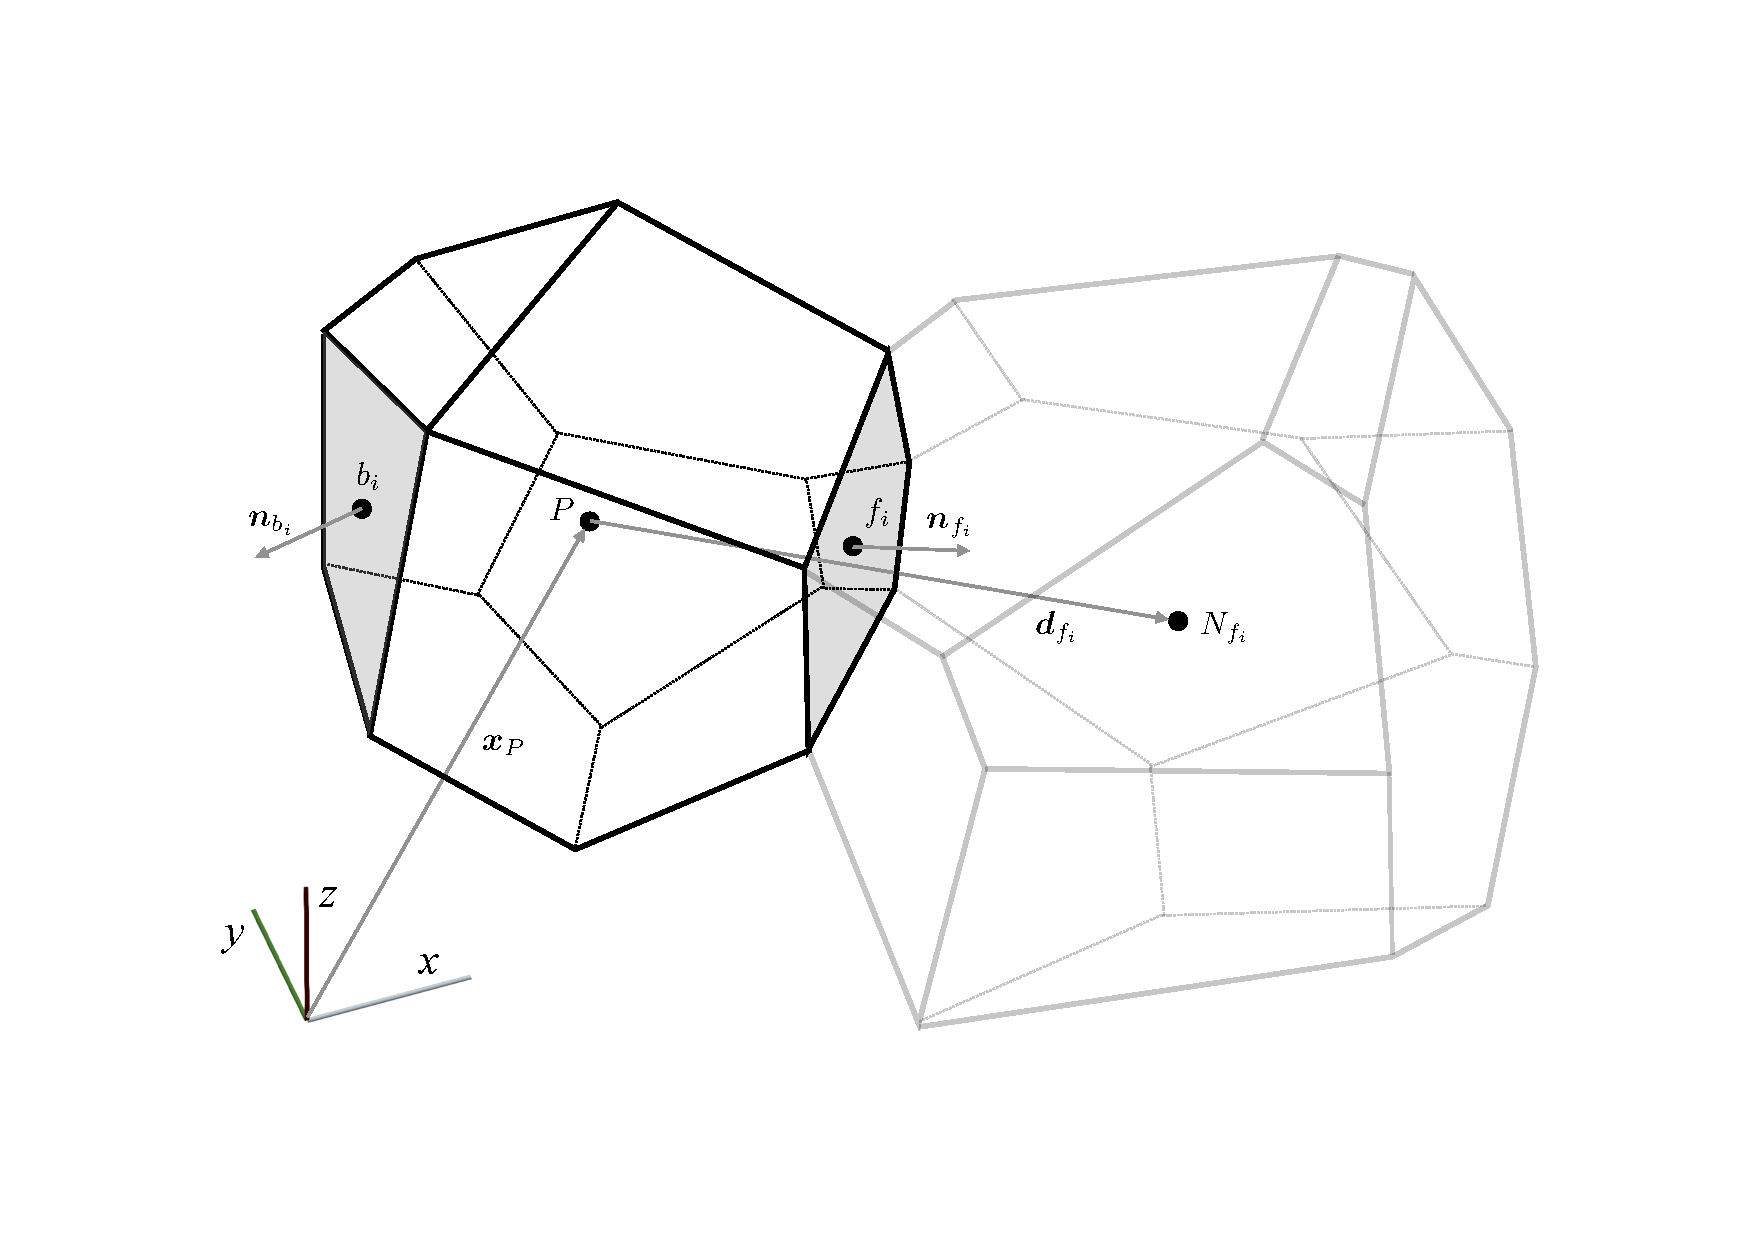
\includegraphics[width=0.8\textwidth]{figures/cell} 
%	\caption{Representative convex polyhedral cell $P$ and neighbouring cell $N_{f_i}$, which share a face $f_i$ (Taken from \citet{Cardiff2025:JFNK})}
%	\label{fig:cell}
%\end{figure}
%
%
%
%
%
%
%
%%%--------------------------------------------------------------------------------------------------------------------%%
%\subsection{Newton-Type Solution Method}
%%%--------------------------------------------------------------------------------------------------------------------%%
%To facilitate the application of a Newton-type solution algorithm, the governing equations are expressed in \emph{residual} form as:
%\begin{eqnarray} \label{eqn:residual}
%	    \bb{R}(\bb{v}) =
%	         \begin{pmatrix}
%			\bb{R}_u  \\
%			R_p \\
%			\bb{R}_m \\
%		    	\bb{R}_d
%		    \end{pmatrix}
%		= \bb{0}
%\end{eqnarray}
%where $\bb{R}$ represents the \emph{residual} (imbalance) of the equations, which is a function of the primary unknowns field $\bb{v} = \left\{\bb{v}, p, \bb{d}_m, \bb{d} \right\}$.
%Concretely, the components of the residual are given as \hl{use on Omega f notation etc}
%\begin{eqnarray} \label{eq:residuals}
%    \bb{R}_u %(\bb{v})
%    &=&
%	\oint_{\Gamma^f_0}  \left[ J^\Gamma (\bb{F}^\Gamma)^{-\text{T}} \cdot \hat{\bb{n}}_0^f \right]
%		\cdot \left[\nu (\bb{F}^\Gamma)^{-T} \cdot \left( \bb{\nabla}_0 \bb{v}^f \right) \right] \, d\Gamma^f_0
%	+ \int_{\Omega^f_0} J^\Gamma (\bb{F}^\Gamma)^{-T} \cdot \left( \bb{\nabla}_0 p \right) \, d\Omega^f_0 \notag \\
%	&&+ \int_{\Omega^f_0} \bb{f}_{b_0}^f \, d\Omega^f_0
%	- \int_{\Omega^f_0} J^\Gamma \frac{\partial \bb{v}^f}{\partial t} \, d\Omega^f_0 
%	- \oint_{\Gamma^f_0}  \left[ J^\Gamma (\bb{F}^\Gamma)^{-\text{T}} \cdot \hat{\bb{n}}_0^f \right] \cdot \left(\bb{v}^f - \frac{\partial \bb{d}_m}{\partial t}\right) \bb{v}^f \, d\Gamma^f_0
%	\notag \\
%	&&+\; \bb{\mathcal{D}}_v
%	\notag \\
%    R_p %(\bb{v})
%    &=&	\oint_{\Gamma^f_0}  \left[ J^\Gamma (\bb{F}^\Gamma)^{-\text{T}}  \cdot \hat{\bb{n}}_0^f \right] \cdot \bb{v}^f \, d\Gamma^f_0 \;+\; \mathcal{D}_p
%    \notag \\
%    \bb{R}_m
%    &=&
%    \oint_{\Gamma_0^f} \bb{n}_0^f \cdot
%    \left[
%    \mu^\Gamma \bb{\nabla}_0 \bb{d}_m + \mu^\Gamma \left(\bb{\nabla}_0 \bb{d}_m \right)^T
%    + \lambda^\Gamma (\bb{\nabla}_0 \cdot \bb{d}_m) \textbf{I}
%    \right]
%    \, d\Gamma_0^f
%    \;+\; \bb{\mathcal{D}}_m
%    \notag \\
%    \bb{R}_d %(\bb{v})
%    &=&
%    \oint_{\Gamma_0^s} \left( J \bb{F}^{-\text{T}} \cdot \bb{n}_0^s \right) \cdot \bb{\sigma}^s \ d\Gamma_0^s
%    + \int_{\Omega_0^s}  \bb{f}_{b_0}^s \, d\Omega_0^s
%    - \int_{\Omega_0^s} \rho_0 \frac{\partial^2 \bb{d} }{\partial t^2} \; d\Omega_0^s
%    \;+\; \bb{\mathcal{D}}_d
%\end{eqnarray}
%where $\bb{\mathcal{D}}_v$, $\mathcal{D}_p$, $\bb{\mathcal{D}}_m$, and $\bb{\mathcal{D}}_d$ are stabilisation terms to be defined.
%
%The residuals $\bb{R}_v$, $R_p$ and $\bb{R}_m$ are applied to each cell in the fluid domain and discretised, while residual $\bb{R}_d$ is applied to each cell in the solid domain and discretised, as is described below.
%The resulting system of coupled nonlinear equations in terms of $\bb{v}$ can be linearised and iteratively solved using a Newton-type method:
%%In Newton-type methods, a Taylor expansion about a current point $\bb{u}_k$ can be used to solve Equation \ref{eqn:residual} \cite{Knoll2004}:
%%\begin{eqnarray}
%%	\bb{R}(\bb{u}_{k+1}) = \bb{R}(\bb{u}_{k}) \;+\;  \bb{R}'(\bb{u}_{k}) (\bb{u}_{k+1} - \bb{u}_{k}) \;+\; \text{H.O.T.} = \bb{0}
%%\end{eqnarray}
%%Neglecting the higher-order terms ($\text{H.O.T.}$) yields the strict Newton method in terms of an iteration over a sequence of linear systems: 
%\begin{eqnarray} \label{eq:NewtonRaphson}
%	\bb{J}(\bb{v}_k) \delta \bb{v} &=& -\bb{R}(\bb{v}_k), \notag \\
%	\bb{v}_{k+1} &=& \bb{v}_k + s \, \delta \bb{v}, \notag \\
%	\quad
%	k &=& 0,1,...
%\end{eqnarray}
%where $\bb{J} \equiv \bb{R}' \equiv \partial \bb{R}/\partial \bb{v}$ is the Jacobian matrix.
%Starting the Newton procedure requires the specification of $\bb{v}_0$.
%%is iteratively solved by linearisation about the current value of the solution, leading to a linear system and iterative update of the solution vector:
%%\begin{eqnarray}
%%    \label{eq:NewtonRaphsonA}
%%    \overbrace{\left[ \frac{\partial \mathcal{R}(\bb{u})}{\partial \bb{u}} \right]_n}^{\mathcal{J}} \Delta \bb{u} = -\mathcal{R}(\bb{u})_n \\
%%    \label{eq:NewtonRaphsonB}
%%    \bb{u}_{n+1} = \bb{u}_{n} + \alpha \Delta \bb{u}
%%\end{eqnarray}
%%where subscript $n$ indicates the outer (Newton) iteration index.
%The scalar $s > 0$ can be chosen to improve convergence, for example, using a line search or under-relaxation/damping procedure, and is equal to unity in the classic Newton-Raphson approach.
%Iterations are performed over this system until the residual $\bb{R}(\bb{v}_k)$ and solution correction $\delta \bb{v}$ are sufficiently small, with appropriate normalisation.
%
%The linear system in Equation \ref{eq:NewtonRaphson} can be represented as
%\begin{eqnarray} \label{eqn:jacobian}
%\begin{bmatrix}
%%\bb{J}_{vv} & \bb{J}_{vp} & \bb{J}_{vm} & \bb{J}_{vd} \\
%%J_{pv} & J_{pp} & J_{pm} & J_{pd} \\
%\bb{J}_{vv} & \bb{J}_{vp} & \bb{J}_{vm} & 0 \\
%J_{pv} & J_{pp} & J_{pm} & 0 \\
%0 & 0 & \bb{J}_{mm} & \bb{J}_{md} \\
%\bb{J}_{dv} & \bb{J}_{dp} & 0 & \bb{J}_{dd}
%\end{bmatrix}_k
%\begin{bmatrix}
%\delta \bb{v} \\
%\delta p \\
%\delta \bb{d}_m \\
%\delta \bb{d}
%\end{bmatrix}
%=
%-
%\begin{bmatrix}
%\bb{R}_v  \\
%R_p \\
%\bb{R}_m \\
%\bb{R}_d
%\end{bmatrix}_k
%\end{eqnarray}
%where the subscript $k$ indicates that the Jacobian matrix and right-hand side vector are evaluated in terms of $\bb{v}_k$.
%\hl{Jvd and Jpd can be removed since this comes form Jvm and Jpm}
%The submatrices $\bb{J}_{ab}$ represent the coupling in the residual $a$ coming from the unknown $b$.
%Several types of coupling exist between the residual components:
%\begin{itemize}
%	\item \textbf{Fluid-to-solid}, represented by $\bb{J}_{dv}$ and $\bb{J}_{dp}$:
%	the fluid forces are passed to the solid by replacing the solid stress $\bb{\sigma}^s$ with the fluid stress $\bb{\sigma}^f$ at the fluid-solid interface in $\bb{R}_d$.
%	\item \hl{Merge with below}  \textbf{Solid-to-fluid}, represented by $\bb{J}_{vd}$ and $\bb{J}_{pd}$ \hl{not required, per se}
%	the solid motion is passed to the fluid equations by replacing the fluid velocity $\bb{v}^f$ by the solid velocity $\nicefrac{\partial \bb{d}^s}{\partial t}$ at the fluid-solid interface in $\bb{R}_v$ and $R_p$.
%	\item \textbf{Solid-to-mesh}, represented by $\bb{J}_{md}$:
%	the solid motion is passed to the fluid mesh by replacing the fluid mesh displacement $\bb{d}_m$ by the solid displacement $\bb{d}^s$ at the fluid-solid interface in $\bb{R}_m$. 
%	\item \hl{Rename} \textbf{Mesh-to-fluid}, represented by $\bb{J}_{vm}$ and $\bb{J}_{pm}$:
%	the fluid mesh motion velocity $\nicefrac{\partial \bb{d}_m}{\partial t}$ appears in the advection term of $\bb{R}_v$ and the fluid mesh motion displacement $\bb{d}_m$ appears in the fluid mesh deformation gradients terms ($\bb{F}_m$, $J_m$) of $\bb{R}_v$ and $R_p$.
%\end{itemize}
%Several submatrices are not present, indicating an absence of coupling:
%\begin{itemize}
%	\item $\bb{J}_{mv}$, $\bb{J}_{mp}$: the fluid mesh motion $\bb{d}_m$ does not depend on the fluid velocity $\bb{v}$ and pressure $p$.
%	\item $\bb{J}_{dm}$: the solid motion $\bb{d}$ does not depend on the fluid mesh motion $\bb{d}_m$. 
%\end{itemize}
%
%The current work adopts a Jacobian-free Newton-Krylov solution procedure \citep{Cardiff2025JFNK} to solve the nonlinear system given by Equation \ref{eqn:residual}.
%Consequently, the true Jacobian given in Equation \ref{eqn:jacobian} is not strictly required; instead, an approximate Jacobian $\tilde{\bb{J}}$ is formed and employed to precondition the nonlinear Newton-Krylov solution.
%Note that adopting an approximate Jacobian does not affect the final converged solution in each time step, assuming convergence is achieved; in addition, the quadratic convergence of the Newton-Raphson method is unaffected, once again assuming convergence is achieved.
%Instead, this approximate Jacobian only affects the convergence of the linear iterative (Krylov) solver.
%Others have proposed the use of physics-specific preconditioning procedures, e.g. \citet{Gee20??_Wall} and \citet{Heil2008} => these approaches sound better, but here we use a simpler approach to demonstrate the first FVM monolithic FSI solver.
%Physics preconditioners are certainly suitable (e.g., using SIMPLE and segregated solvers) and will be examined in a future publication.
%Here, the approximate Jacobian $\tilde{\bb{J}}$ takes the form:
%\begin{eqnarray} \label{eqn:approx_jacobian}
%\tilde{\bb{J}} =
%\begin{bmatrix}
%%\tilde{\bb{J}}_{vv} & \bb{J}_{vp} & \bb{J}_{vm} & \bb{J}_{vd} \\
%%J_{pv} & \tilde{J}_{pp} & J_{pm} & J_{pd} \\
%\tilde{\bb{J}}_{vv} & \bb{J}_{vp} & \tilde{\bb{J}}_{vm} & 0 \\
%\bb{J}_{pv} & \tilde{J}_{pp} & 0 & 0 \\
%0 & 0 & \tilde{\bb{J}}_{mm} & \tilde{\bb{J}}_{md} \\
%0 & \bb{J}_{dp} & 0 & \tilde{\bb{J}}_{dd}
%\end{bmatrix}_k
%\end{eqnarray}
%where $\bb{J}_{dv}$ is dropped as the fluid viscous forces on the fluid-solid interface are assumed to be small in comparison to the fluid pressure forces (represented by $\bb{J}_{dp}$).
%In addition, compact stencil approximate Jacobians for solid ($\tilde{\bb{J}}_{dd}$), fluid ($\tilde{\bb{J}}_{vv}$, $\tilde{J}_{pp}$) and fluid mesh motion ($\tilde{\bb{J}}_{mm}$, $\tilde{\bb{J}}_{md}$) terms are employed.
%The $J_{pm}$ term is also ignored, and $\tilde{\bb{J}}_{vm}$ contains only the advective mesh velocity term.
%
%Details of the cell-centred finite volume discretisation of residuals are given below, in addition to calculating the approximate Jacobian submatrices.
%
%
%
%
%%%--------------------------------------------------------------------------------------------------------------------%%
%\subsection{Cell-Centred Finite Volume Discretisation Principles}
%%%--------------------------------------------------------------------------------------------------------------------%%
%\hl{This section summaries the main principles of the cell-centred FV scheme employed here}
%\hl{State truncated Taylor series}
%A nominally second-order cell-centred finite volume discretisation is employed in this work.
%This section describes the adopted finite volume discretisation for general volume and surface integrals, gradient calculation, and time derivatives.
%Equation-specific details are given in the subsequent fluid dynamics, mesh motion and solid dynamics sections.
%
%The presented discretisation is second-order accurate in space for displacement if the cell-centred displacement gradients (and the stress) are at least first-order accurate in space, even if the cell faces are not flat.
%
%To quell zero-energy solution modes (i.e. checkerboarding oscillations), Rhie-Chow-type stabilisation terms \cite{Rhie1983} are added to the residual equations, as described below.
%As shown in \citet{Cardiff2025jfnk} and \citet{Cardiff2020}, a Rhie-Chow-type stabilisation term can be cast in the same form as an upwind stabilisation term.
%
%%%The conservation equation (Equations \ref{eqn:momentum_lingeom}, \ref{eqn:momentum_TL}, or \ref{eqn:momentum_UL}) is applied to each cell $\mathcal{P}$ and discretised in terms of the displacement at the centroid of the cell $\bb{u}_P$ and the displacements at the centroids of the neighbouring cells $\bb{u}_{N_{f_i}} \in N_i$.
%%The conservation equation (Equations \ref{eqn:momentum_lingeom}, \ref{eqn:momentum_TL}, or \ref{eqn:momentum_UL}) is applied to each cell $P$ and discretised in terms of the displacement at the centroid of the cell $\boldsymbol{u}_P$ and the displacements $\boldsymbol{u}_{N_{f_i}}$ at the centroids of the neighbouring cells.
%%% $\boldsymbol{u}_{N_{f_i}} \in \mathcal{U}_{\mathcal{N}_P}$, where $\mathcal{U}_{\mathcal{N}_P}$ represents the set of such displacements.
%%Proceeding with the discretisation, the volume and surface integrals in the governing equation are approximated by algebraic equations as described below.
%
%%%----------------------------%%
%\paragraph{Volume Integrals}
%%%----------------------------%%
%%To discretise the volume integrals, the integrand $\bb{\phi}$ is assumed to locally vary according to a truncated Taylor series expansion about the centroid of cell $P$:
%%\begin{eqnarray}
%%	\bb{\phi}(\bb{x})  \approx \bb{\phi}_P + (\bb{x} - \bb{x}_P) \cdot \nabla \bb{\phi}_P
%%\end{eqnarray}
%%where subscript $P$ indicates a value at the centroid of the cell $P$.
%%% assuming a linear variation of the integrand across the cell, the mid-point rule approximates the integral in terms of the cell centre value.
%%Consequently,
%Volume integrals over a cell $P$ are approximated to second-order accuracy by assuming the integrand $\bb{\phi}$ to vary locally according to a truncated Taylor series expansion about the centroid:
%\begin{eqnarray} \label{eq:volume_integral}
%	\int_{\Omega_P} \bb{\phi} \, d \Omega_P
%		&\approx& \int_{\Omega_P}  \left[ \bb{\phi}_P + (\bb{x} - \bb{x}_P) \cdot \nabla \bb{\phi}_P \right] d \Omega_P \notag \\
%%		&\approx& \int_{\mathrm{\Omega}}  \bb{\phi}_P d\mathrm{\Omega}  + \int_{\mathrm{\Omega}}  (\bb{x} - \bb{x}_P) \cdot \nabla \bb{\phi}_P d\mathrm{\Omega} \notag \\
%		&\approx& \bb{\phi}_P \Omega_P
%\end{eqnarray}
%where subscript $P$ indicates a value at the centroid of the cell $P$, $\Omega_P$ is the volume of cell $P$ and $\int_{\Omega_P} (\bb{x} - \bb{x}_P) d\Omega_P \equiv 0$ by definition of the cell centroid.
%This approximation corresponds to the midpoint rule and one-point quadrature.
%
%
%%%----------------------------%%
%\paragraph{Surface Integrals}
%%%----------------------------%%
%%In the current work, discretisation of the surface integrals (in Equations \ref{eq:residuals}) depends on whether the terms are diffusion-type (e.g., $\bb{n} \cdot \bb{\sigma}^s$, $\bb{n} \cdot \left(\nu \bb{\nabla} \bb{v}\right)$) or advection-type term (e.g., $\bb{n} \cdot \bb{v}$).
%%Surface integral terms require the surface integration of terms containing the derivative of a solution unknown in the deformed configuration (e.g., $\bb{\nabla} \bb{v}$), while advection-type terms contain solution unknown in the deformed configuration (e.g., $\bb{\nabla} \cdot \left(\bb{v} \otimes \bb{v}\right)$, $\bb{\nabla} \cdot \bb{v}$).
%Surface integrals of generic integrand $\bb{q}$ can be discretised using one-point quadrature at each face as
%\begin{eqnarray} \label{eq:diffusion_discret}
%	\oint_{\Gamma_P} \bb{n} \cdot \bb{q}  \; d\Gamma_P
%	&=& \sum_{f_i \in \mathcal{F}_P} \int_{\Gamma_{f_i}} \bb{n} \cdot \bb{q}  \,  d \Gamma_{f_i} \notag \\
%	&\approx&
%%	\sum_{f_i \in \mathcal{F}_P^{\text{int}} \cup \mathcal{F}_P^{\text{disp}} \cup \mathcal{F}_P^{\text{symm}}} \bb{\Gamma}_{f_i} \cdot \bb{q}_{f_i}
%%	\sum_{f_i \in \mathcal{F}_P^{\text{non-trac}}} \bb{\Gamma}_{f_i} \cdot \bb{q}_{f_i}
%	\sum_{f_i \in \mathcal{F}_P^{\text{int}}} \bb{\Gamma}_{f_i} \cdot \bb{q}_{f_i}
%	+ \sum_{d_i \in \mathcal{F}_P^{\text{D}}} \bb{\Gamma}_{d_i} \cdot \bb{q}_{P}
%	+ \sum_{s_i \in \mathcal{F}_P^{\text{symm}}} \bb{\Gamma}_{s_i} \cdot \bb{q}_{s_i}
%	+ \sum_{t_i \in \mathcal{F}_P^{\text{trac}}} |\bb{\Gamma}_{t_i}| \bar{\bb{Q}}_{t_i}
%\end{eqnarray}
%where $\Gamma_P$ indicates the surface of cell $P$, $\bb{\Gamma}_{f_i}$ indicates the deformed area vector of face $f_i$, and $\bar{\bb{Q}}_{t_i}$ represents the prescribed normal component of $\bb{q}$ on a boundary faces where $\bb{q}$ is prescribed, e.g. $\bar{\bb{Q}}_{t_i}$ represents the prescribed traction on fluid and solid Neumann boundaries.
%%where $\Gamma_P$ indicates the surface of cell $P$, and $\bb{\Gamma}_{f_i}$ indicates the area vector of face $f_i$.
%
%%As solution unknowns ($\bb{v}$, $p$, $\bb{d}_m$, $\bb{d}$) are assumed to vary linearly within each cell, their gradients are constant within each cell.
%In the current work, a unique definition of solution gradient (e.g., $\bb{q}_{f_i}$)
%In the current work, the value of the integrand $\bb{q}$ at each cell face $f_i$ is given as a weighted-averaged of values in the two cells straddling the face \citep{Cardiff2025JFNK, Jasak1996}:
%%The stress $\bb{\sigma}_{f_i}$ at an internal face is calculated by linear interpolation from the adjacent cell centres \citep{Jasak1996}:
%\begin{eqnarray}
%	\label{eq:face_interp}
%	\bb{q}_{f_i} &=& w_{f_i} \bb{q}_P + (1 - w_{f_i}) \bb{q}_{N_{f_i}} \\
%	\bb{q}_{f_i} &=& \left( \nicefrac{1}{2} \right) \left[ \bb{q}_P +  \bb{q}_{N_{f_i}} \right] \\
%%	\left(\bb{\nabla} \bb{\phi}\right)_{f_i} &=& w_{f_i} \left(\bb{\nabla} \bb{\phi}\right)_P + (1 - w_{f_i}) \left(\bb{\nabla} \bb{\phi}\right)_{N_{f_i}} \\
%%	\left(\bb{\nabla} \bb{\phi}\right)_{f_i} &=& \left( \nicefrac{1}{2} \right) \left[ \left(\bb{\nabla} \bb{\phi}\right)_P +  \left(\bb{\nabla} \bb{\phi}\right)_{N_{f_i}} \right]
%%	\left(\bb{\nabla} \bb{\phi}\right)_{f_i} &=& \nicefrac{\left[ \left(\bb{\nabla} \bb{\phi}\right)_P +  \left(\bb{\nabla} \bb{\phi}\right)_{N_{f_i}} \right]}{2}
%	\label{eq:face_interp_weights}
%	w_{f_i} &=& (\bb{n}_{f_i} \cdot [\bb{x}_{N_{f_i}} - \bb{x}_{f_i}])/(\bb{n}_{f_i} \cdot [\bb{x}_{N_{f_i}} - \bb{x}_{P} ])
%\end{eqnarray}
%%where $\bb{\sigma}_{f_i}$ is the stress at an interface face $f_i$, 
%where $w_{f_i}$ is the interpolation weight a face $f_i$. % is defined as $w_{f_i} = (\bb{n}_{f_i} \cdot [\bb{x}_{N_{f_i}} - \bb{x}_{f_i}])/(\bb{n}_{f_i} \cdot [\bb{x}_{N_{f_i}} - \bb{x}_{P} ])$.
%% however, achieving second-order accuracy of the displacement field is independent of the value of the weights, and, for example, $w_{f_i} = \nicefrac{1}{2}$ would also be sufficient.
%\hl{We can average instead for derivative terms - 2nd eq}
%\hl{Should I use deformed config weights?}
%\hl{Mat props harmonic interp?}
%
%%It is noted that the displacement is assumed to vary linearly within each cell; hence, the displacement gradient and stress are constant within each cell.
%
%The integrand value $\bb{q}_{s_i}$  at a symmetry boundary face is calculated as
%\begin{eqnarray} \label{eq:symm}
%	\bb{q}_{s_i} 
%%		&=& \frac{1}{2} \left (\bb{q}_P + \bb{R}_{s_i} \cdot \bb{q}_{P} \right) \notag \\
%		&=& \left( \nicefrac{1}{2} \right) \left (\bb{q}_P + \bb{R}_{s_i} \cdot \bb{q}_{P} \right) \notag \\
%		&=& \left (\textbf{I} - \bb{n}_{s_i} \otimes \bb{n}_{s_i} \right) \cdot \bb{q}_P
%\end{eqnarray}
%where $\bb{R}_{s_i} \cdot \bb{q}_{P}$ represents the mirror reflection of $\bb{q}_P$ across the symmetry boundary face $s_i$.
%The reflection tensor is $\bb{R}_{s_i} = \textbf{I} - 2 \bb{n}_{s_i} \otimes \bb{n}_{s_i}$ \citep{Demirdzic2022}, with $\bb{n}_{s_i}$ indicating the unit normal of the symmetry boundary face $s_i$.
%%From Equation \ref{eq:symm}, it is clear that shear stresses are zero on a symmetry plane boundary face.
%%Note from Equation \ref{eq:divStressDiscret} that the stress on displacement boundary faces is assumed to be equal to the stress $\bb{\sigma}_P$ at the centroid of cell $P$.
%
%The discretisation of surface integral terms above (Equation \ref{eq:diffusion_discret}) is given in terms of deformed configuration;
%integration over the initial domain is achieved by expressing the deformed area vectors $\bb{\Gamma}_{f_i}$ at a face in terms of the initial configuration:
%\begin{eqnarray} 
%	\bb{\Gamma}_{f_i} = J_{f_i} \bb{F}_{f_i}^{-\text{T}} \cdot \bb{\Gamma}_{0_{f_i}}
%\end{eqnarray} 
%where the face values $J_{f_i}$ and $\bb{F}_{f_i}^{-\text{T}}$ are averaged from adjacent cells according to Equation \ref{eq:face_interp}.
%\hl{Use text(T) for all transposes}
%
%%An exception to the surface integral discretisation above is made for the advection term in the fluid linear momentum equation, which is instead discretised as \hl{fix}
%%\begin{eqnarray} \label{eq:advect_discret}
%%	\oint_{\Gamma_P} \bb{n} \cdot \left(\bb{v} - \frac{\partial \bb{d}_{m}}{\partial t}\right) \bb{v} \; d\Gamma_P
%%	&=& \sum_{f_i \in \mathcal{F}_P} \int_{\Gamma_{f_i}} \bb{n} \cdot  \left(\bb{v} - \frac{\partial \bb{d}_{m}}{\partial t}\right) \bb{v}   \,  d \Gamma_{f_i} \notag \\
%%	&\approx&
%%	\sum_{f_i \in \mathcal{F}_P^{\text{int}}} \bb{\Gamma}_{f_i} \cdot \left( \bb{v}_{f_i} - \frac{\partial \bb{d}_{m,f_i}}{\partial t} \right) \tilde{\bb{v}}_{f_i} \notag \\
%%	&&+ \sum_{d_i \in \mathcal{F}_P^{\text{D}}} \bb{\Gamma}_{d_i} \cdot \left( \bb{v}_{d_i} - \frac{\partial \bb{d}_{m,d_i}}{\partial t} \right) \tilde{\bb{v}}_{d_i}
%%	%+ \sum_{s_i \in \mathcal{F}_P^{\text{symm}}} \bb{\Gamma}_{s_i} \cdot \bb{p}_{s_i}
%%%	+ \sum_{t_i \in \mathcal{F}_P^{\text{trac}}} |\bb{\Gamma}_{t_i}| \bar{\bb{P}}_{t_i}
%%\end{eqnarray}
%%%where $\tilde{\bb{v}}_{f_i}$ is interpolated using upwinding.
%%Note that the advection term is zero at symmetry faces as the face flux (mass flow) is zero by definition.
%%Here, $\tilde{\bb{v}}_{f_i}$ is calculated using first-order upwind for the approximate Jacobian $\bb{J}_v$ contribution
%%\begin{eqnarray}
%%	\tilde{\bb{v}}_{f_i} =
%%		\text{max}\left[ \bb{\Gamma}_{f_i} \cdot \left( \bb{v}_{f_i} - \frac{\partial \bb{d}_{m,f_i}}{\partial t} \right), \, 0\right] \tilde{\bb{v}}_P
%%		+ \text{min}\left[ \bb{\Gamma}_{f_i} \cdot \left( \bb{v}_{f_i} - \frac{\partial \bb{d}_{m,f_i}}{\partial t} \right), \, 0\right] \tilde{\bb{v}}_{N_i}
%%\end{eqnarray}
%%where $\text{max}\left[\cdot \,, \cdot \right]$ is the maximum operator and $\text{min}\left[\cdot \,, \cdot \right]$ is the minimum operator.
%%In the residual $\bb{R}_v$ (which controls the order of accuracy of the final solution), $\tilde{\bb{v}}_{f_i}$ is calculated using a second-order \hl{upwind/CD/limited-decide} scheme:
%%\begin{eqnarray}
%%	\tilde{\bb{v}}_{f_i} =  w_{f_i} \bb{v}_P + (1 - w_{f_i}) \bb{v}_{N_{f_i}}
%%\end{eqnarray}
%
%
%
%%%----------------------------%%
%\paragraph{Gradients}
%%%----------------------------%%
%Cell-centred displacement gradients $\bb{\nabla} \bb{\phi}$ are determined using a weighted first-neighbours least squares method \citep{Cardiff2025JFNK, Jasak1996}: \hl{introduce symbol for LS vec}
%\begin{eqnarray} \label{eq:leastSquaresGrad}
%	\left(\bb{\nabla}\bb{\phi}\right)_P
%		&=&\sum_{f_i \in \mathcal{F}^{\text{int}}_P} w_{f_i} |\bb{\Gamma}_{f_i}| \frac{\bb{G}^{-1}_P \cdot \bb{d}_{f_i}}{\bb{d}_{f_i} \cdot \bb{d}_{f_i}}  \otimes \left(\bb{\phi}_{N_{f_i}} - \bb{\phi}_P \right) \notag \\
%		&&+ \sum_{d_i \in \mathcal{F}^{\text{D}}_P} w_{f_i} |\bb{\Gamma}_{d_i}| \frac{ \bb{G}^{-1}_P \cdot \bb{d}_{d_i} }{\bb{d}_{d_i} \cdot \bb{d}_{d_i}} \otimes \left(\bb{\phi}_{d_i} - \bb{\phi}_P \right) \notag \\
%		&&+ \sum_{s_i \in \mathcal{F}^{\text{symm}}_P} w_{f_i} |\bb{\Gamma}_{s_i}| \frac{\bb{G}^{-1}_P \cdot \bb{d}_{s_i}}{\bb{d}_{s_i} \cdot \bb{d}_{s_i}} \otimes \left(\bb{R}_{s_i} \cdot \bb{\phi}_P - \bb{\phi}_P \right)
%\end{eqnarray}
%which is exact for linear functions.
%The tensor multiplication operator $\otimes$ is replaced with an appropriate vector-scalar multiplication operator when $\bb{\phi}$ is a scalar, e.g. kinematic pressure $p$.
%%where the least squares weights are $\omega_{f_i} = 1/|\bb{d}_{f_i}|$ and  $\omega_{b_i} = 1/|\bb{d}_{b_i}|$.
%The vector $\bb{\phi}_{b_i}$ indicates the value of $\bb{\phi}$ at the centroid of boundary face ${b_i}$, while vector $\bb{d}_{d_i}$ connects the centroid of cell $P$ to the centroid of displacement boundary face $d_i$.
%The quantity $\bb{R}_{s_i} \cdot \bb{\phi}_P$ represents the mirror reflection of $\bb{\phi}_P$ across the symmetry boundary face $s_i$.
%% where the reflection tensor is $\bb{R}_{s_i} = \textbf{I} - 2 \bb{n}_{s_i} \otimes \bb{n}_{s_i}$ \citep{Demirdzic2022}.
%The vector $\bb{d}_{s_i}$ connects the centroid $\bb{x}_P$ of cell $P$ with its mirror reflection $\bb{R}_{s_i}  \cdot \bb{x}_P$ through boundary face $s_i$.
%
%%Traction boundary faces are excluded in Equation \ref{eq:leastSquaresGrad}, as the displacement is unknown there; this is in contrast to the default approach in OpenFOAM \citep{Jasak2011}.
%The $\bb{G}_P$ tensor for cell $P$ is calculated as
%\begin{eqnarray}
%	 \bb{G}_P &=&
%%	 \sum_{{f_i} \in \mathcal{F}^{\text{int}}_P} \omega_{f_i}^2 \bb{d}_{f_i} \bb{d}_{f_i}
%%	 +  \sum_{{b_i} \in \mathcal{F}^{\text{disp}}_P} \omega_{b_i}^2 \bb{d}_{b_i} \bb{d}_{b_i}
%%	 +  \sum_{{b_i} \in \mathcal{F}^{\text{symm}}_P} \omega_{b_i}^2 \bb{d}_{b_i}^{\text{symm}} \bb{d}_{b_i}^{\text{symm}}
%%	 \sum_{{f_i} \in \mathcal{F}^{\text{int}}_P} \frac{\bb{d}_{f_i} \otimes \bb{d}_{f_i}}{\bb{d}_{f_i} \cdot \bb{d}_{f_i}}
%%	 +  \sum_{{d_i} \in \mathcal{F}^{\text{disp}}_P} \frac{\bb{d}_{d_i} \otimes \bb{d}_{d_i}}{\bb{d}_{d_i} \cdot \bb{d}_{d_i}}
%%	 +  \sum_{{s_i} \in \mathcal{F}^{\text{symm}}_P} \frac{\bb{d}_{s_i} \otimes \bb{d}_{s_i}}{\bb{d}_{s_i} \cdot \bb{d}_{s_i}}
%	 \sum_{{f_i} \in \mathcal{F}^{\text{int}}_P} (1 - w_{f_i}) |\bb{\Gamma}_{f_i}|  \frac{\bb{d}_{f_i} \otimes \bb{d}_{f_i}}{\bb{d}_{f_i} \cdot \bb{d}_{f_i}} \notag \\
%	 &&+  \sum_{{d_i} \in \mathcal{F}^{\text{disp}}_P} (1 - w_{d_i}) |\bb{\Gamma}_{d_i}|  \frac{\bb{d}_{d_i} \otimes \bb{d}_{d_i}}{\bb{d}_{d_i} \cdot \bb{d}_{d_i}} \notag \\
%	 && +  \sum_{{s_i} \in \mathcal{F}^{\text{symm}}_P} (1 - w_{s_i}) |\bb{\Gamma}_{s_i}|  \frac{\bb{d}_{s_i} \otimes \bb{d}_{s_i}}{\bb{d}_{s_i} \cdot \bb{d}_{s_i}}
%\end{eqnarray}
%As the $w |\bb{\Gamma}| \ \bb{G}^{-1}_P \cdot \bb{d}/(\bb{d}\cdot \bb{d})$ vectors in Equation \ref{eq:leastSquaresGrad} are purely a function of the mesh, they can be computed once (or each time the mesh moves) and stored.
%Equation \ref{eq:leastSquaresGrad} approximates the cell-centre gradients to at least a first-order accuracy, increasing to second-order accuracy on certain smooth grids \citep{Syrakos2023};
%first-order accurate gradients are sufficient to preserve second-order accuracy of the cell-centre primary unknowns.
%
%
%
%%%----------------------------%%
%\paragraph{Time Derivatives}
%%%----------------------------%%
%Time derivatives $\nicefrac{\partial \bb{\phi}}{\partial t}$ at the centre of cell $P$ are discretised in time using the second-order backwards (BDF2) scheme:
%\begin{eqnarray} \label{eq:ddt}
%	\left(\frac{\partial \bb{\phi}}{\partial t}\right)_P^{[t+1]}
%		&\approx& \frac{3 \bb{\phi}_P^{[t+1]} - 4 \bb{\phi}_P^{[t]} + \bb{\phi}_P^{[t-1]}}{2\Delta t} 
%\end{eqnarray}
%where $\Delta t$ is the time increment -- assumed constant here.
%Superscript $[t]$ indicates the time level, with $\bb{\phi}_P^{[t+1]}$ corresponding to the value of $\bb{\phi}$ at the centre of cell $P$ at the current time step $[t+1]$.
%Using the second-order backwards scheme, second time derivatives $\nicefrac{\partial^2 \bb{\phi}}{\partial t^2}$ are discretised as
%\begin{eqnarray}
%	\left(\frac{\partial^2 \bb{\phi}}{\partial t^2}\right)_P
%	&\approx&
%	\frac{3\left( 
%		\dfrac{3\bb{\phi}_P^{[t+1]} - 4\bb{\phi}_P^{[t]} + \bb{\phi}_P^{[t-1]}}{2\Delta t} 
%		\right) 
%	- 4\left(\frac{\partial \bb{\phi}}{\partial t}\right)_P^{[t]} + \left(\frac{\partial \bb{\phi}}{\partial t}\right)_P^{[t-1]}}{2\Delta t}
%\end{eqnarray}
%where the $\frac{\partial \bb{\phi}}{\partial t}$ terms are discretised are also discretised using the second-order backwards scheme (Equation \ref{eq:ddt}).
%
%
%
%%%--------------------------------------------------------------------------------------------------------------------%%
%\subsection{Discretisation of the Residuals and Jacobian}
%%%--------------------------------------------------------------------------------------------------------------------%%
%
%
%%%--------------------------------------------------------------------------------------------------------------------%%
%\subsubsection[Fluid Dynamics Residuals Discretisation]{Fluid Dynamics Discretisation}
%%%--------------------------------------------------------------------------------------------------------------------%%
%This section describes the discretisation of the fluid residuals $\bb{R}_v$ and $R_p$, as well as the defining the adopted approximate Jacobian submatrices $\bb{J}_{vv}$, $\bb{J}_{vp}$, $J_{pp}$ and $J_{pv}$.
%
%The fluid equation linear momentum residual $\bb{R}_v$ repeated here is
%\begin{eqnarray}
%    \bb{R}_u %(\bb{v})
%    &=&
%	\oint_{\Gamma^f_0}  \left[ J^\Gamma (\bb{F}^\Gamma)^{-\text{T}} \cdot \hat{\bb{n}}_0^f \right]
%		\cdot \left[\nu (\bb{F}^\Gamma)^{-T} \cdot \left( \bb{\nabla}_0 \bb{v}^f \right) \right] \, d\Gamma^f_0
%	+ \int_{\Omega^f_0} J^\Gamma (\bb{F}^\Gamma)^{-T} \cdot \left( \bb{\nabla}_0 p \right) \, d\Omega^f_0 \notag \\
%	&&+ \int_{\Omega^f_0} \bb{f}_{b_0}^f \, d\Omega^f_0
%	- \int_{\Omega^f_0} J^\Gamma \frac{\partial \bb{v}^f}{\partial t} \, d\Omega^f_0 
%	- \oint_{\Gamma^f_0}  \left[ J^\Gamma (\bb{F}^\Gamma)^{-\text{T}} \cdot \hat{\bb{n}}_0^f \right] \cdot \left(\bb{v}^f - \frac{\partial \bb{d}_m}{\partial t}\right) \bb{v}^f \, d\Gamma^f_0
%\end{eqnarray}
%
%The three volume integrals are approximated to second-order accuracy using the mid-point rule (Equation \ref{eq:volume_integral}):
%\begin{eqnarray}
%	\int_{\Omega^f_0} J^\Gamma (\bb{F}^\Gamma)^{-T} \cdot \left( \bb{\nabla}_0 p \right) \, d\Omega^f_0
%		&\approx& J^\Gamma_P (\bb{F}^\Gamma_P)^{-T} \cdot \left( \bb{\nabla}_0 p \right)_P  \Omega_{0,P} \\
%	\int_{\Omega^f_0} \bb{f}_{b_0}^f \, d\Omega^f_0	&\approx&		\left( \bb{f}_{b_0}^f \right)_P  \Omega_{0,P} \\
%	\int_{\Omega^f_0} J^\Gamma \frac{\partial \bb{v}^f}{\partial t} \, d\Omega^f_0
%		&\approx& 	J^\Gamma_P  \frac{3 \bb{v}_P - 4 \bb{v}_P^{[t]} + \bb{v}_P^{[t-1]}}{2\Delta t}  \Omega_{0,P}
%\end{eqnarray}
%where the second-order in time backwards differencing scheme is used for the time derivative;
%the $[t+1]$ time index notation is dropped for brevity, i.e., $\bb{v}_P  \equiv \bb{v}_P^{[t+1]}$.
%The cell-centred pressure gradient $\left( \bb{\nabla}_0 p \right)_P$ is calculated using weighted least squares (Equation \ref{eq:least_squares}).
%The cell-centred fluid mesh deformation gradient and its determinant are calculated in terms of the fluid mesh displacement gradient according to Equation \ref{eq:fluid_deformation_grad}, where the cell-centred gradient is calculated using weighted least squares (Equation \ref{eq:least_squares}).
%
%The diffusion (viscous stresses) surface integral is approximated as \hl{FSI-term}
%\begin{align}
%	\oint_{\Gamma^f_0}  \left[ J^\Gamma (\bb{F}^\Gamma)^{-\text{T}} \cdot \hat{\bb{n}}_0^f \right]
%		\cdot & \left[\nu (\bb{F}^\Gamma)^{-T} \cdot \left( \bb{\nabla}_0 \bb{v}^f \right) \right] \, d\Gamma^f_0
%		\approx \notag \\
%		& \sum_{f_i \in \mathcal{F}^{\text{int}}_P}
%		\left[ J^\Gamma_{f_i} (\bb{F}^\Gamma_{f_i})^{-\text{T}} \cdot \hat{\bb{\Gamma}}_{0, f_i}^f \right]
%			\cdot \left[\nu_{f_i} (\bb{F}^\Gamma_{f_i})^{-T} \cdot \left( \bb{\nabla}_0 \bb{v}^f \right)_{f_i} \right]
%%			\notag \\
%%		+ \sum_{d_i \in \mathcal{F}^{\text{D}}_P} TODO \notag \\
%%		+ \sum_{s_i \in \mathcal{F}^{\text{symm}}_P} TODO 
%\end{align}
%The face values $J^\Gamma_{f_i}$, $\bb{F}^\Gamma_{f_i}$, $\nu_{f_i}$, and $\left( \bb{\nabla}_0 \bb{v}^f \right)_{f_i} $ are interpolated from the cell-centres using Equation \ref{eq:interp}.
%Once again, the cell-centred gradient is calculated using weighted least squares (Equation \ref{eq:least_squares}).
%
%The advection surface integral is approximated as \hl{FSI-term}
%\begin{align}
%	\oint_{\Gamma^f_0}  \left[ J^\Gamma (\bb{F}^\Gamma)^{-\text{T}} \cdot \hat{\bb{n}}_0^f \right]
%		& \cdot \left(\bb{v}^f - \frac{\partial \bb{d}_m}{\partial t}\right) \bb{v}^f \, d\Gamma^f_0
%		\approx \notag \\
%		& \sum_{f_i \in \mathcal{F}_P^{\text{int}}}
%	\left[ J^\Gamma_{f_i} (\bb{F}^\Gamma_{f_i})^{-\text{T}} \cdot \hat{\bb{\Gamma}}_{0, f_i}^f \right]
%		\cdot \left( \bb{v}_{f_i} - \frac{3 \bb{d}_{m,f_i} - 4 \bb{d}_{m,f_i}^{[t]} + \bb{d}_{m,f_i}^{[t-1]}}{2\Delta t}  \right) \tilde{\bb{v}}_{f_i} \notag \\
%	&+ \sum_{d_i \in \mathcal{F}_P^{\text{D}}} \left[ J^\Gamma_{d_i} (\bb{F}^\Gamma_{d_i})^{-\text{T}} \cdot \hat{\bb{\Gamma}}_{0, d_i}^f \right]
%		 \cdot \left( \bb{v}_{d_i} - \frac{\partial \bb{d}_{m,d_i}}{\partial t} \right) \tilde{\bb{v}}_{d_i}
%\end{align}
%%Note that the advection term is zero at symmetry faces as the face flux (mass flow) is zero by definition.
%Note that the advection term is zero at the fluid-solid interface as the face flux (mass flow) is zero by definition.
%Here, $\tilde{\bb{v}}_{f_i}$ is calculated using first-order upwind for the approximate Jacobian $\bb{J}_v$ contribution \hl{make consistent with Jacobian section later}
%\begin{eqnarray} \label{eq:advection_velocity_interp}
%	\tilde{\bb{v}}_{f_i} =
%		\text{max}\left[ \psi_{f_i}, \, 0\right] \bb{v}_P + \text{min}\left[ \psi_{f_i}, \, 0\right] \bb{v}_{N_i}
%\end{eqnarray}
%where $\text{max}\left[\cdot \,, \cdot \right]$ is the maximum operator and $\text{min}\left[\cdot \,, \cdot \right]$ is the minimum operator.
%The volume flux $\psi$ through the control volume face is $\psi = \left( J_m \bb{F}_m^{-\text{T}} \cdot \bb{\Gamma}_0 \right) \cdot \left(\bb{v} - \frac{\partial \bb{d}_m}{\partial t} \right)$.
%In the residual $\bb{R}_v$ (which controls the order of accuracy of the final solution), $\tilde{\bb{v}}_{f_i}$ is calculated using a second-order \hl{upwind/CD/limited-decide} scheme:
%\begin{eqnarray}
%	\tilde{\bb{v}}_{f_i} =  w_{f_i} \bb{v}_P + (1 - w_{f_i}) \bb{v}_{N_{f_i}}
%\end{eqnarray}
%
%The vector stabilisation term $\bb{\mathcal{D}}_v$ takes the form of the difference between a compact and large stencil gradient at a cell face:
%\begin{eqnarray}
%	\bb{\mathcal{D}}_v
%	&=& \sum_{f_i \in \mathcal{F}^{\text{int}}_P} \alpha_v \nu \left[
%		\left|\bb{\Delta}_{0,f_i} \right| \frac{ \bb{v}_{N_{f_i}} - \bb{v}_P}{\left|\bb{\delta}_{0,f_i}\right|}	- \bb{\Delta}_{0,f_i} \cdot \left(\bb{\nabla}_0 \bb{v} \right)_{f_i}
%		\right]    \left|\bb{\Gamma}_{0,f_i}\right|
%\end{eqnarray}
%where $\alpha_v$ is a user parameter for controlling the amount of stabilisation ($\alpha_v = 0$ gives no stabilisation, $\alpha_v > 0$ gives stabilisation).
%
%
%
%The diagonal block ($3\times3$ for 3-D, $2\times2$ for 2-D) for cell $P$ (row $P$, column $P$) is: \hl{consistent with JFNK paper, but we can do better by including J/F}
%\begin{align}
%    	\left\{ \tilde{\bb{J}}_{vv} \right\}_{PP} =&
%	- \sum_{f_i \in \mathcal{F}^{\text{int}}_P} \alpha_v \nu
%	\frac{ \left|\bb{\Delta}_0 \right| }{\left|\bb{\delta}_0 \right|}  \left|\bb{\Gamma}_0 \right| \textbf{I} \notag \\
%	& - \; \frac{3}{2} \frac{J_m \Omega_{0,P}}{\Delta t} \textbf{I}
%	\;\;\; - \; \sum_{f_i \in \mathcal{F}^{\text{int}}_P}
%	\max \left[\psi_{f_i}, 0\right] \textbf{I} + w_{f_i} \left( H_P \bb{v}_P + H_Q \bb{v}_Q \right) \otimes \mathbf{\Gamma}_{f_i}
%\end{align}
%%\emph{over-relaxed} 
%where the vectors $\bb{\Delta}_0 = \nicefrac{\bb{\delta}_{0,m}}{\bb{\delta}_{0,m} \cdot \bb{n}_{0,m}}$.
%The Heaviside function terms are defined as
%\begin{eqnarray}
%	H_P &=& H(\psi_{f_i}) =
%	\begin{cases}
%		1  & \text{if} \quad \psi_{f_i} > 0 \\
%		0  & \text{otherwise}
%	\end{cases} \notag \\
%	H_Q &=& 1 - H(\psi_{f_i})
%\end{eqnarray}
%%where $\text{max}\left[\cdot\,,\, \cdot\right]$ is the maximum operator and $\text{min}\left[\cdot\,,\, \cdot\right]$ is the minimum operator.
%while the off-diagonal contribution (row $P$, column $Q \neq P$) is
%\begin{eqnarray}
%    	\left\{ \tilde{\bb{J}}_{vv} \right\}_{PQ} &=&
%	\nu \frac{ \left|\bb{\Delta}_0 \right| }{\left|\bb{d}_0 \right|}  \left|\bb{\Gamma}_0 \right| \textbf{I}
%	\;\; + \;\; \min \left[\psi_{f_i}, 0\right] \textbf{I} + (1 - w_{f_i}) \left( H_P \bb{v}_P + H_Q \bb{v}_Q \right) \otimes \mathbf{\Gamma}_{f_i}
%\end{eqnarray}
%
%The block ($3\times1$ for 3-D, $2\times1$ for 2-D) diagonal coefficient for cell $P$ (row $P$, column $P$) for Jacobian submatrix $\bb{J}_{vp}$ is
%\begin{eqnarray}
%	\left\{
%	\tilde{\bb{J}}_{vp} 
%	\right\}_{PP}
%	&=& \sum_{f_i \in \mathcal{F}^{\text{int}}_P} J_{P,m} \, \bb{g}_{P,f_i} \,  \Omega_{0,P}
%\end{eqnarray}
%where $\bb{g}_{P, f_i}$ is the least squares vector stored for cell $P$ at face $f_i$, as defined in Equation \ref{eq:least_squares_vectors}.
%While the off-diagonal contribution (row $P$, column $Q \neq P$) is
%\begin{eqnarray}
%	\left\{
%	\tilde{\bb{J}}_{vp} 
%	\right\}_{PQ}
%	&=& -J_{P,m} \, \bb{g}_{P,f_i} \,  \Omega_{0,P}
%\end{eqnarray}
%
%
%The coupling matrix $\bb{J}_{vm} \equiv \partial \bb{R}_{v}/\partial \bb{d}_m$ accounts for the effect of the fluid mesh motion on the fluid momentum equation.
%This effect comes in two \hl{three? FSI velocity} forms: firstly, the mesh velocity directly appears in the advection term; secondly, all terms contain $\bb{F}_m$ and $J_m$, which map the terms from the initial fluid mesh to the unknown deformed mesh.
%The block ($3\times3$ for 3-D, $2\times2$ for 2-D) diagonal coefficient for cell $P$ (row $P$, column $P$) is expressed as
%\begin{eqnarray}
%	 \left[ \tilde{\bb{J}}_{vm} \right]_{PP} &=&
%		 \frac{\alpha_t}{\Delta t} \sum_{f_i \in \mathcal{F}^{\text{int}}_P}
%		 \left(J_m \bb{F}_m^{-\text{T}} \cdot \bb{\Gamma}_m \right)_{f_i} \otimes \tilde{\bb{v}}_{f_i}
%%	 \left[ \tilde{\bb{J}}_{vm} \right]_{PP} &=&
%%	 \begin{cases}
%%		\sum_{f_i \in \mathcal{F}^{\text{int}}_P}  \left(J_m \bb{F}_m^{-T} \cdot \bb{\Gamma} \right)_{f_i}^{[m]} \otimes \bb{v}_F
%%		& \text{if } \Phi > 0, \\
%%		\sum_{f_i \in \mathcal{F}^{\text{int}}_P}  \left(J_m \bb{F}_m^{-T} \cdot \bb{\Gamma} \right)_{f_i}^{[m]} \otimes \bb{v}_F
%%		& \text{otherwise}.
%%	\end{cases}
%\end{eqnarray}
%where $\tilde{\bb{v}}_{f_i}$ is defined in Equation \ref{eq:advection_velocity_interp}.
%For the first-order Euler scheme $\alpha_t = 1$, while for the second-order backward scheme $\alpha_t = \nicefrac{3}{2}$.
%The off-diagonal coefficients (row $P$, column $Q \neq P$) are
%\begin{eqnarray}
%	 \left[ \tilde{\bb{J}}_{vm} \right]_{PQ} &=&
%	 	 \frac{\alpha_t}{\Delta t} \left(J_m \bb{F}_m^{-\text{T}} \cdot \bb{\Gamma}_m \right)_{PQ}^{[m]} \otimes \tilde{\bb{v}}_{f_i}
%%	 \begin{cases}
%%		\left(J_m \bb{F}_m^{-T} \cdot \bb{\Gamma} \right)_{f_i}^{[m]} \otimes \bb{v}_P
%%		& \text{if } \Phi > 0, \\
%%		\left(J_m \bb{F}_m^{-T} \cdot \bb{\Gamma} \right)_{f_i}^{[m]} \otimes \bb{v}_Q
%%		& \text{otherwise}.
%%	\end{cases}
%\end{eqnarray}
%where subscript $PQ$ indicates a quantity associated with the internal face $f$ shared between cells $P$ and $Q$.
%
%
%
%Moving to the pressure equation, the fluid continuity equation residual $R_p$ repeated here is
%\begin{eqnarray}
%    R_p    &=&	\oint_{\Gamma^f_0}  \left[ J^\Gamma (\bb{F}^\Gamma)^{-\text{T}}  \cdot \hat{\bb{n}}_0^f \right] \cdot \bb{v}^f \, d\Gamma^f_0 \;+\; \mathcal{D}_p
%\end{eqnarray}
%
%The velocity divergence term is approximated for cell $P$ as
%\begin{eqnarray}
%	\oint_{\Gamma^f}  \left[ J_m \bb{F}_m^{-\text{T}}  \cdot \hat{\bb{n}}_0 \right] \cdot \bb{v} \, d\Gamma_0
%	&\approx&
%		\sum_{f_i \in \mathcal{F}^{\text{int}}_P}
%		\left( J_m \bb{F}_m^{-\text{T}}  \cdot \hat{\bb{\Gamma}}_0 \right)
%		\cdot \left[ w_{f_i} \bb{v}_P + (1 - w_{f_i})\bb{v}_{N_{f_i}}  \right]
%\end{eqnarray}
%where the linear interpolation weights $w_{f_i}$ are given by Equation \ref{eq:face_interp_weights}.
%
%The scalar stabilisation term $\mathcal{D}_p$ takes the same form as the vector stabilisation $\mathcal{D}_v$, and is calculated as \hl{use Hiro's alpha damping} \hl{ref vs def config?}:
%\begin{eqnarray}
%	\mathcal{D}_p
%	&=& \sum_{f_i \in \mathcal{F}^{\text{int}}_P} \alpha_p D_p \left[
%		\left|\bb{\Delta}_{0,f_i} \right| \frac{ p_{N_{f_i}} - p_P}{\left|\bb{\delta}_{0,f_i}\right|}	- \bb{\Delta}_{0,f_i} \cdot \left(\bb{\nabla}_0 p \right)_{f_i}
%		\right]    \left|\bb{\Gamma}_{0,f_i}\right|
%\end{eqnarray}
%where, like $\alpha_v$, $\alpha_p$ is a user parameter for controlling the amount of stabilisation.
%
%%\hl{J-pp}
%The approximate Jacobian submatrix $\tilde{J}_{pp}$ is derived from the compact stencil term of the stabilisation $\mathcal{D}_p$.
%The block ($1\times1$ for 3-D and 2-D) diagonal coefficient for cell $P$ (row $P$, column $P$) is
%\begin{eqnarray}
%	\left\{ \tilde{J}_{pp} \right\}_{PP} &=&
%		- \sum_{f_i \in \mathcal{F}^{\text{int}}_P}  \alpha_p D_p
%		\frac{ \left|\bb{\Delta}_{0,f_i} \right| }{\left|\bb{\delta}_{0,f_i}\right|}    \left|\bb{\Gamma}_{0,f_i}\right|
%\end{eqnarray}
%while the off-diagonal coefficient (row $P$, column $Q \neq P$) is
%\begin{eqnarray}
%	\left\{ \tilde{J}_{pp} \right\}_{PQ}	 &=&
%		\alpha_p D_p \frac{ \left|\bb{\Delta}_{0,f_i} \right| }{\left|\bb{\delta}_{0,f_i}\right|}    \left|\bb{\Gamma}_{0,f_i}\right|
%\end{eqnarray}
%
%
%%\hl{J-pv}
%For the approximate Jacobian submatrix $\tilde{\bb{J}}_{pv}$, the block ($1\times3$ for 3-D, $1\times2$ in 2-D) diagonal coefficient for cell $P$ (row $P$, column $P$) is
%\begin{eqnarray}
%	\left\{ \tilde{\bb{J}}_{pv} \right\}_{PP}	&=&
%		\sum_{f_i \in \mathcal{F}^{\text{int}}_P} w_{f_i}  J_{m,f_i} \bb{F}_{m,f_i}^{-\text{T}}  \cdot \hat{\bb{\Gamma}}_{0,f_i}
%\end{eqnarray}
%while the off-diagonal contribution is
%\begin{eqnarray}
%	\left\{ \tilde{\bb{J}}_{pv} \right\}_{PQ} &=&
%		(1 - w_{f_i})  J_{m,f_i} \bb{F}_{m,f_i}^{-\text{T}}  \cdot \hat{\bb{\Gamma}}_{0,f_i}
%\end{eqnarray}
%
%
%
%
%
%
%%%----------------------------%%
%\subsubsection[Discretisation of the Solid Dynamics Residual]{Discretisation of the Solid Dynamics Residual $\bb{R}_d$}
%%%----------------------------%%
%The solid linear momentum equation residual $\bb{R}_d$ repeated here is
%\begin{eqnarray}
%    \bb{R}_d
%    &=&
%    \oint_{\Gamma_0^s} \left( J \bb{F}^{-\text{T}} \cdot \bb{n}_0^s \right) \cdot \bb{\sigma}^s \ d\Gamma_0^s
%    + \int_{\Omega_0^s}  \bb{f}_{b_0}^s \, d\Omega_0^s
%    - \int_{\Omega_0^s} \rho_0 \frac{\partial^2 \bb{d} }{\partial t^2} \; d\Omega_0^s
%    \;+\; \bb{\mathcal{D}}_d
%\end{eqnarray}
%
%The two volume integrals are approximated to second-order accuracy using the mid-point rule (Equation \ref{eq:volume_integral}):
%\begin{eqnarray}
%	\int_{\Omega_0^s} \rho_0 \frac{\partial^2 \bb{d} }{\partial t^2} \; d\Omega_0^s
%		\;&\approx&\; \frac{\rho_{0,P}}{2\Delta t}
%		\left[
%			3\left( 
%			\dfrac{3\boldsymbol{d}_P - 4\boldsymbol{d}_P^{[t]} + \boldsymbol{d}_P^{[t-1]}}{2\Delta t} 
%			\right) 
%			- 4\boldsymbol{v}_P^{[t]} + \boldsymbol{v}_P^{[t-1]}
%		\right] \Omega_{0,P} \\
%	\int_{\Omega_0^s}  \bb{f}_{b_0}^s \, d\Omega_0^s
%		\;&\approx&\;  \rho_{0,P} \left(\bb{f}^s_{b_0}\right)_P \Omega_{0,P}
%\end{eqnarray}
%where the acceleration term has been approximated using the second-order in time backwards differencing (BDF2) scheme.
%Here, $\boldsymbol{v} = \nicefrac{\partial \bb{u}}{\partial t}$ refers to the solid velocity vector (not to be confused with the fluid velocity vector), also calculated using the BDF2 scheme:
% \begin{eqnarray}
%	\boldsymbol{v}_P^{[t+1]}	&\approx&
%		\dfrac{3\boldsymbol{u}_P^{[t+1]} - 4\boldsymbol{u}_P^{[t]} + \boldsymbol{u}_P^{[t-1]}}{2\Delta t} 
%\end{eqnarray}
%
%
%
%The surface integral term, corresponding to the divergence of stress is discretised as
%\begin{align} \label{eq:divStressDiscret}
%	\oint_{\Gamma_0^s} \left( J \bb{F}^{-\text{T}} \cdot \bb{n}_0^s \right) \cdot \bb{\sigma}^s & \, d\Gamma_0^s
%	\approx  \sum_{f_i \in \mathcal{F}_P^{\text{int}}} \left( J_{f_i} \bb{F}^{-\text{T}}_{f_i} \cdot \bb{\Gamma}_{0,f_i}^s \right) \cdot \bb{\sigma}_{f_i} \notag \\
%	&+ \sum_{d_i \in \mathcal{F}_P^{\text{disp}}} \bb{\Gamma}_{d_i} \cdot \bb{\sigma}_{P}
%%	+ \sum_{s_i \in \mathcal{F}_P^{\text{symm}}} \bb{\Gamma}_{s_i} \cdot \bb{\sigma}_{s_i}
%	+ \sum_{t_i \in \mathcal{F}_P^{\text{trac}}} |\bb{\Gamma}_{t_i}| \bar{\bb{T}}_{t_i}
%\end{align}
%where vector $\bar{\bb{T}}_{t_i}$ represents the prescribed traction on the traction boundary face $t_i$.
%For faces $f_i$ in Equation \ref{eq:divStressDiscret} that are on traction boundary faces $b_i \in \mathcal{F}_P^{\text{trac}} \subset \mathcal{F}_P$, 
%the traction $\bar{\bb{t}}_{b_i}$ is known and is directly enforced; that is, $\bb{\Gamma}_{f_i} \cdot \bb{\sigma}_{f_i} = |\bb{\Gamma}_{f_i}| \bb{n}_{f_i} \cdot \bb{\sigma}_{f_i} =  |\bb{\Gamma}_{f_i}| \bar{\bb{t}}_{b_i}$.
%%subscript $f$ indicates a quantity at the centre of a cell face, and 
%The stress $\bb{\sigma}_{f_i}$ at an internal face is calculated by linear interpolation from the adjacent cell centres (Equation \ref{eq:interp}).
%%Vector $\bb{d}_{f}$ connects cell centre $P$ with cell centre $N_f$, $\bb{d}_f = \bb{x}_{N_f} - \bb{x}_P$, and $\bb{n}_{f}$ is the outward-facing unit normal to the face $f$.
%%Similarly, the stress $\bb{\sigma}_{s_i}$ at a symmetry boundary face is calculated as
%%\begin{eqnarray} \label{eq:symm}
%%	\bb{\sigma}_{s_i}
%%		&=& \frac{1}{2} \left (\bb{\sigma}_P + \bb{R}_{s_i} \cdot \bb{\sigma}_{P} \right) \notag \\
%%		&=& \left (\textbf{I} - \bb{n}_{s_i} \otimes \bb{n}_{s_i} \right) \cdot \bb{\sigma}_P
%%\end{eqnarray}
%%where $\bb{R}_{s_i} \cdot \bb{\sigma}_{P}$ represents the mirror reflection of $\bb{\sigma}_P$ across the symmetry boundary face $s_i$.
%%The reflection tensor is $\bb{R}_{s_i} = \textbf{I} - 2 \bb{n}_{s_i} \otimes \bb{n}_{s_i}$ \citep{Demirdzic2022}, with $\bb{n}_{s_i}$ indicating the unit normal of the symmetry boundary face $s_i$.
%%From Equation \ref{eq:symm}, it is clear that shear stresses are zero on a symmetry plane boundary face.
%Note from Equation \ref{eq:divStressDiscret} that the stress on displacement boundary faces is assumed to be equal to the stress $\bb{\sigma}_P$ at the centroid of cell $P$.
%
%\hl{Fluid traction on FSI interface}
%
%The cell-centred stress $\bb{\sigma}_P$ is calculated as a function of the displacement gradient according to the chosen mechanical law, for example, as shown in Appendix \ref{app:mechLaws}.
%
%
%The stabilisation term  $\bb{\mathcal{D}}_{d,P}$ for a cell $P$ takes the following form \hl{two d: new symbol} \hl{deformed config?}:
%\begin{eqnarray} \label{eq:RhieChow}
%	\bb{\mathcal{D}}_{d,P}
%	&=& \sum_{f_i \in \mathcal{F}^{\text{int}}_P} \alpha \bar{K}_{f_i} \left[
%		\left|\bb{\Delta}_{f_i} \right| \frac{ \bb{d}_{N_{f_i}} - \bb{d}_P}{\left|\bb{\delta}_{f_i}\right|}	- \bb{\Delta}_{f_i} \cdot \left(\bb{\nabla} \bb{d} \right)_{f_i}
%		\right]    \left|\bb{\Gamma}_{f_i}\right| \notag \\
%	&&+ \sum_{d_i \in \mathcal{F}^{\text{disp}}_P} \alpha \bar{K}_{d_i} \left[
%		\left|\bb{\Delta}_{d_i} \right| \frac{ \bar{\bb{u}}_{d_i} - \bb{u}_P}{\left|\bb{\delta}_{d_i}\right|}	- \bb{\Delta}_{d_i} \cdot \left(\bb{\nabla} \bb{d} \right)_{P}
%		\right]    \left|\bb{\Gamma}_{d_i}\right| %\notag \\
%%	&&+ \sum_{s_i \in \mathcal{F}^{\text{symm}}_P} \alpha \bar{K}_{s_i} \left[
%%		\left|\bb{\Delta}_{s_i} \right| \frac{ \bb{R}_{s_i} \cdot \bb{d}_{P} - \bb{d}_P}{\left|\bb{d}_{s_i}\right|} - \bb{\Delta}_{s_i} \cdot \left(\bb{\nabla} \bb{d} \right)_{s_i}
%%		\right]    \left|\bb{\Gamma}_{s_i}\right|
%\end{eqnarray}
%%which comes from the difference between Equations \ref{eq:diffusion} and \ref{eq:diffusion_exp}.
%where $\alpha_d > 0$ is a user-defined parameter for globally scaling the amount of stabilisation, similar to $\alpha_v$ and $\alpha_p$.
%Parameter $\bar{K}$ is a stiffness-type parameter that gives the stabilisation an appropriate scale and dimension, chosen here to be $\bar{K} = \frac{4}{3}\mu + \kappa = 2\mu + \lambda$ following previous work \cite{Jasak2000, Cardiff2017, Cardiff2018}, where $\mu$ is the shear modulus (first Lam\'{e} parameter), $\kappa$ is the bulk modulus, and $\lambda$ is the second Lam\'{e} parameter (or their equivalent for the chosen mechanical law).
%Vector $\bar{\bb{d}}_{d_i}$ represents the prescribed displacement at the centroid of displacement boundary face $d_i$.
%%where $N_f$ represents the set of faces $f$ in cell $P$, and neighbouring cell centre $N_f$ shares face $f$ with the cell $P$.
%%Vector $\bb{n}_{f}$ is the outward-facing unit normal to the face $f$.
%%The quantities $\bb{\Delta} = \nicefrac{\bb{d}}{\bb{d} \cdot \bb{n}}$ are termed the \emph{over-relaxed orthogonal} vectors \cite{Jasak1996}.
%The displacement gradient $\left(\bb{\nabla} \bb{d} \right)_{f_i}$ at the internal face $f_i$ is calculated by interpolation from adjacent cell centres (like in Equation \ref{eq:stressInterp}).
%%Similarly, the displacement gradient $\left(\bb{\nabla} \bb{d} \right)_{s_i}$ at a symmetry boundary face $s_i$ is averaged from cell $P$ and its mirror reflection across face $s_i$, as in Equation \ref{eq:symm}.
%Note that the displacement gradient at the displacement boundary $d_i$ is assumed to be equal to the displacement gradient at the centroid of cell $P$.
%In addition, no stabilisation term is applied on a traction boundary face $t_i$.
%
%
%
%%The true Jacobian $\bb{J}_{dd} \equiv \partial \bb{R}_{dd}/\partial \bb{d}$;
%In the current work, an approximate Jacobian $\tilde{\bb{J}}_{dd}$ is employed for the solid dynamics based on the segregated solution procedures commonly employed in cell-centred finite volume solid dynamics.
%A recent article \citep{Cardiff2025jfnk} by the authors describes this approach in detail.
%The approximate Jacobian $\tilde{\bb{J}}_{dd}$ is derived from the inertia term and the compact stencil component of the stabilisation term $\bb{\mathcal{D}}_d$.
%%\begin{eqnarray}
%%	\tilde{\bb{J}}_{dd}
%%	&=&
%%	\frac{\partial}{\partial \bb{u}} \left[ \oint_{\Gamma_P} \alpha \bar{K} \, \bb{n} \cdot \bb{\nabla} \bb{u} \; d\Gamma_P
%%	 \; -\;  \int_{\Omega_P} \rho \frac{\partial^2 \bb{u} }{\partial t^2} \, d\Omega_P \right]
%%\end{eqnarray}
%%The linearised system (Equation \ref{eq:Seg}) is formed for each cell in the domain, resulting in a system of algebraic equations:
%%\begin{eqnarray} \label{eq:SegSys}
%%    \left[ \bb{\tilde{J}} \right]  \; \left[ \delta \bb{u} \right] = - \left[\bb{R}(\bb{u}_k)\right]
%%\end{eqnarray}
%The $M_d \times M_d$ matrix $\left[ \bb{\tilde{J}}_{dd} \right]$ is symmetric, where $M = 3|\mathcal{P}^s|$ in 3-D and $M = 2|\mathcal{P}^s|$ in 2-D.
%%If $\Delta t < \infty$ or $\mathcal{F}^{\text{disp}}_P \neq \emptyset$, matrix $\left[ \bb{\tilde{J}}_{dd} \right]$ is strongly diagonally dominant; otherwise, it is weakly diagonally dominant.
%The block ($3\times3$ for 3-D, $2\times2$ for 2-D) diagonal coefficient for cell $P$ (row $P$, column $P$) is
%\begin{eqnarray}
%	 \left[ \tilde{\bb{J}}_{dd} \right]_{PP} &=&
%		- \sum_{f_i \in \mathcal{F}^{\text{int}}_P}  \alpha \bar{K}
%		\frac{ \left|\bb{\Delta}_{f_i} \right| }{\left|\bb{\delta}_{f_i}\right|}    \left|\bb{\Gamma}_{f_i}\right| \textbf{I} 
%	    \quad-  \sum_{d_i \in \mathcal{F}^{\text{disp}}_P}  \alpha \bar{K}
%%		\left|\bb{\Delta}_{d_i} \right| \left( \ \frac{ \bar{\bb{u}}_{d_i} - \bb{u}_P}{\left|\bb{d}_{d_i}\right|}  \right) 
%		 \frac{ \left|\bb{\Delta}_{d_i} \right| }{\left|\bb{\delta}_{d_i}\right|} 
%		\left|\bb{\Gamma}_{d_i}\right| \textbf{I} %\notag \\
%%	 &&\quad - \sum_{s_i \in \mathcal{F}^{\text{symm}}_P} \alpha \bar{K}
%%		 \frac{ \left|\bb{\Delta}_{s_i} \right|}{\left|\bb{d}_{s_i}\right|}
%%		\left|\bb{\Gamma}_{s_i}\right|  \bb{n}_{s_i} \otimes \bb{n}_{s_i} 
%	\quad- \quad \frac{9}{4}  \frac{\rho_P \Omega_P}{\Delta t^2} \textbf{I}
%\end{eqnarray}
%while the off-diagonal coefficients (row $P$, column $Q \neq P$) are
%\begin{eqnarray}
%	\left[\tilde{\bb{J}}_{dd} \right] _{PQ} &=&
%		\alpha \bar{K} \frac{ \left|\bb{\Delta}_{f_{PQ}} \right| }{\left|\bb{d}_{f_{PQ}}\right|} \left|\bb{\Gamma}_{f_{PQ}}\right| \textbf{I} 
%\end{eqnarray}
%where subscript $PQ$ indicates a quantity associated with the internal face $f$ shared between cells $P$ and $Q$.
%
%
%
%The coupling matrix $\bb{J}_{dp} \equiv \partial \bb{R}_{d}/\partial p$ accounts for the effect of the fluid interface pressure on the solid deformation. 
%The block ($3\times1$ for 3-D, $2\times1$ for 2-D) coefficient for row $P$, column $Q$ is expressed here as
%\begin{eqnarray}
%%	 \left[ \tilde{\bb{J}}_{dp} \right]_{PQ} &=& -\rho^f \bb{\Gamma}_{f_i}^s
%	 \left[ \tilde{\bb{J}}_{dp} \right]_{PQ} &=& -\rho^f \left[ J^s (\bb{F}^s)^{-\text{T}} \cdot \hat{\bb{\Gamma}}_0^s \right] 
%\end{eqnarray}
%for all pairs of fluid-solid cells at the fluid-solid interface, where $P$ indicates the solid cell index (and row of $\bb{J}_{dp}$) and $Q$ indicates the fluid cell index (and column of $\bb{J}_{dp}$).
%Note that the fluid density $\rho^f$ scales the fluid kinematic pressure to actual pressure, and viscous effects are neglected in the approximate Jacobian (but not in the residual $\bb{\mathcal{R}}_d$).
%
%
%
%%%----------------------------%%
%\subsubsection[Discretisation of the Fluid Mesh Motion Residual]{Discretisation of the Fluid Mesh Motion Residual $\bb{R}_m$}
%%%----------------------------%%
%The fluid mesh motion equation residual $\bb{R}_m$ repeated here is \hl{maybe we should use large strain approach - see if required in test cases}
%\begin{eqnarray}
%    \bb{R}_m
%    &=&
%    \oint_{\Gamma_0^f} \bb{n}_0^f \cdot
%    \left[
%    \mu^\Gamma \bb{\nabla}_0 \bb{d}_m + \mu^\Gamma \left(\bb{\nabla}_0 \bb{d}_m \right)^T
%    + \lambda^\Gamma (\bb{\nabla}_0 \cdot \bb{d}_m) \textbf{I}
%    \right]
%    \, d\Gamma_0^f
%    \;+\; \bb{\mathcal{D}}_m
%\end{eqnarray}
%
%The discretisation of the stress divergence is
%\begin{align}
%    \oint_{\Gamma_0^f} \bb{n}_0^f \cdot
%    &\left[
%    \mu^\Gamma \bb{\nabla}_0 \bb{d}_m + \mu^\Gamma \left(\bb{\nabla}_0 \bb{d}_m \right)^T
%    + \lambda^\Gamma (\bb{\nabla}_0 \cdot \bb{d}_m) \textbf{I}
%    \right]    \, d\Gamma_0^f
%	\approx \notag \\
%	&\sum_{f_i \in \mathcal{F}_P^{\text{int}}}
%	\bb{\Gamma}_{0,f_i}
%	\cdot
%	\left[
%	\mu_m \left(\bb{\nabla}_0 \bb{d}_m\right)_{f_i} + \mu_m \left(\bb{\nabla}_0 \bb{d}_m \right)^T_{f_i}
%    + \lambda_m (\bb{\nabla}_0 \cdot \bb{d}_m)_{f_i} \textbf{I}
%	\right]
%\end{align}
%where the gradient terms are interpolated from the cell centres to the faces according to Equation \ref{eq:face_interp}.
%
%The vector stabilisation term $\bb{\mathcal{D}}_m$ takes the form as $\bb{\mathcal{D}}_v$:
%\begin{eqnarray}
%	\bb{\mathcal{D}}_m
%	&=& \sum_{f_i \in \mathcal{F}^{\text{int}}_P} \alpha_m (2\mu_m + \lambda_m) \left[
%		\left|\bb{\Delta}_{0,f_i} \right| \frac{ \bb{d}_{m,N_{f_i}} - \bb{d}_{m,P}}{\left|\bb{\delta}_{0,f_i}\right|}	- \bb{\Delta}_{0,f_i} \cdot \left(\bb{\nabla}_0 \bb{d}_m \right)_{f_i}
%		\right]    \left|\bb{\Gamma}_{0,f_i}\right|
%\end{eqnarray}
%
%
%\hl{Merge in text below}
%An additional challenge is that the fluid mesh should be moved (smoothed) to distribute the FSI interface motion throughout the fluid domain.
%To achieve this, the current work adopts a pseudo-solid approach where the fluid mesh is considered to be a solid domain, where the boundary displacements are prescribed.
%The following governing equation is adopted for the fluid mesh motion: \hl{I could add F-old to rotate but keep linear}
%\begin{eqnarray} \label{eqn:motion}
%    \oint_{\tilde{\Gamma}}
%    \bb{n}_u \cdot \left[ \beta_m \mu_m \bb{\nabla}\bb{d}_m
%    + \beta_m \mu_m (\bb{\nabla}\bb{d}_m)^T
%    + \beta_m \lambda_m \text{tr}(\bb{\nabla} \bb{d}_m)\textbf{I} \right] 
%    \, d\tilde{\Gamma}
%    \;=\; \bb{0}
%\end{eqnarray}
%It should be noted that Equation \ref{eqn:motion} is integrated over the fluid reference configuration, but it is not mapped to the deformed configuration; this choice is made purely from an efficiency perspective: the purpose of this equation is merely to maintain fluid mesh quality, and it need not strictly correspond to a physical system.
%To maintain fluid mesh quality near the FSI interface and boundary, the stiffness parameters $\mu_m$ and $\lambda_m$ are defined to be inversely proportional to the distance from the fluid boundary according to:
%\hl{express with if-else}
%\begin{eqnarray}
%	\beta_m &=& \text{min}(\beta_\text{max} \bar{\delta}^{-1}, \text{max}(\beta_\text{min} \bar{\delta}^{-1}, \delta^{-1}))
%\end{eqnarray}
%where $\delta$ is the (approximate) distance from the fluid boundary.
%In the current work, $\delta$ is calculated using a topological search approach, implemented in the \texttt{meshWave} class of OpenFOAM.
%$\beta_m$ is then normalised with respect to its average value, i.e. $\beta_m \coloneqq \frac{\beta_m}{\bar{\beta_m}}$, such that $\bar{\beta_m} \equiv 1$. \hl{introduce additional terms to avoid confusion}
%
%
%%The true Jacobian $\bb{J}_{mm} \equiv \partial \bb{R}_{mm}/\partial \bb{d}_m$; in 
%The current work employs a similar approach for defining an approximate Jacobian $\tilde{\bb{J}}_{mm}$ as is employed for the solid dynamics. based on the segregated solution procedures commonly employed in cell-centred finite volume solid dynamics.
%%A recent article \citep{Cardiff2025jfnk} by the authors describes this approach in detail.
%The approximate Jacobian $\tilde{\bb{J}}_{mm}$ is derived from the compact stencil component of the stabilisation term $\bb{\mathcal{D}}_m$.
%%:
%%\begin{eqnarray}
%%	\tilde{\bb{J}} &=& \frac{\partial}{\partial \bb{d}_m} \left[ \oint_{\Gamma_P} \alpha \bar{K} \, \bb{n} \cdot \bb{\nabla} \bb{d}_m \; d\Gamma_P \right]
%%\end{eqnarray}
%The $M_m \times M_m$ matrix $\left[ \bb{\tilde{J}}_{mm} \right]$ is symmetric and strongly diagonally dominant (due to Dirichlet conditions), where $M_m = 3|\mathcal{P}^f|$ in 3-D and $M_m = 2|\mathcal{P}^f|$ in 2-D.
%The block ($3\times3$ for 3-D, $2\times2$ for 2-D) diagonal coefficient for cell $P$ (row $P$, column $P$) can be expressed as \hl{notation}
%\begin{eqnarray}
%	 \left[ \tilde{\bb{J}}_{mm} \right]_{PP} &=&
%		- \sum_{f_i \in \mathcal{F}^{\text{int}}_P}  \alpha \bar{K}
%		\frac{ \left|\bb{\Delta}_{f_i} \right| }{\left|\bb{\delta}_{f_i}\right|}    \left|\bb{\Gamma}_{f_i}\right| \textbf{I} 
%	    \quad-  \sum_{d_i \in \mathcal{F}^{\text{disp}}_P}  \alpha \bar{K}
%%		\left|\bb{\Delta}_{d_i} \right| \left( \ \frac{ \bar{\bb{u}}_{d_i} - \bb{u}_P}{\left|\bb{d}_{d_i}\right|}  \right) 
%		 \frac{ \left|\bb{\Delta}_{d_i} \right| }{\left|\bb{\delta}_{d_i}\right|} 
%		\left|\bb{\Gamma}_{d_i}\right| \textbf{I} % \notag \\
%%	 &&\quad - \sum_{s_i \in \mathcal{F}^{\text{symm}}_P} \alpha \bar{K}
%%		 \frac{ \left|\bb{\Delta}_{s_i} \right|}{\left|\bb{d}_{s_i}\right|}
%%		\left|\bb{\Gamma}_{s_i}\right|  \bb{n}_{s_i} \otimes \bb{n}_{s_i}
%\end{eqnarray}
%while the off-diagonal coefficients (row $P$, column $Q$) can be expressed as
%\begin{eqnarray}
%	\left[\tilde{\bb{J}}_{mm} \right] _{PQ} &=&
%		\alpha \bar{K} \frac{ \left|\bb{\Delta}_{f_{PQ}} \right| }{\left|\bb{\delta}_{f_{PQ}}\right|} \left|\bb{\Gamma}_{f_{PQ}}\right| \textbf{I} 
%\end{eqnarray}
%where subscript $PQ$ indicates a quantity associated with the internal face $f$ shared between cells $P$ and $Q$.
%
%
%
%
%The true Jacobian $\bb{J}_{md} \equiv \partial \bb{R}_{m}/\partial \bb{d}$; in the current work, an approximate coupling matrix $\tilde{\bb{J}}_{md}$ is employed, where the fluid-solid interface displacement for the fluid mesh interface face is taken as the displacement of the adjacent solid cell centre.
%This results in a small (one-cell) stencil, in contrast to the true Jacobian $\bb{J}_{md}$, which would require a larger stencil due to extrapolation from the adjacent solid cell centre using the solid cell centre displacement gradient.
%
%The block ($3\times3$ for 3-D, $2\times2$ for 2-D) coefficient for row $P$, column $Q$ can be expressed as \hl{ref or current?}
%\begin{eqnarray}
%	 \left[ \tilde{\bb{J}}_{md} \right]_{PQ} &=&
%		\beta_m (2\mu_m + \lambda_m)  \frac{ \left| \bb{\Gamma}_{f_i} \right| }{\bb{n} \cdot \bb{d}_{f_i}}
%\end{eqnarray}
%for all pairs of fluid-solid cells at the fluid-solid interface, where $P$ indicates the fluid cell index (and row of $\bb{J}_{md}$) and $Q$ indicates the solid cell index (and column of $\bb{J}_{md}$).
%
%
%
%%%%%%%%%%%%%%%%%%%%%%%%%%%%%%%%%%%%%%%%%%%%%%%%%%%%%%%%%%%%%%%%%%%
%\section{Solution Algorithms}\label{sec:sol_alg}
%%%%%%%%%%%%%%%%%%%%%%%%%%%%%%%%%%%%%%%%%%%%%%%%%%%%%%%%%%%%%%%%%%%
%
%%- Seg approach summary
%%- JFNK approach summary
%%	- implementation via PETSc. Newton with line search, GMRes with MG preconditioner.
%
%%
%%%%--------------------------------------------------------------------------------------------------------------------%%
%%\subsection{Jacobian-free Newton-Krylov Algorithm}
%%\label{sec:JFNK_alg}
%%%%--------------------------------------------------------------------------------------------------------------------%%
%
%%\hl{2}
%%- preconditioner => important
%%- changes the JFNK approx.
%%- precon affects the JF approx
%
%%The literature indicates that the choice of preconditioner for the inner linearised system has a major impact on the efficiency and robustness of the overall solution procedure.
%The purpose of preconditioning the Jacobian-free Newton-Krylov method is to reduce the number of inner linear solver iterations.
%The current work uses the GMRES linear solver for the inner system.
%
%Concretely, the preconditioner needs to approximately solve the linear system $\bb{y} = \bb{P}^{-1} \bb{v}$.
%%Thus, while we may refer to the matrix P, operationally the algorithm only requires the action of $P^{-1}$ on a vector.
%
%
%In the current work, the PETSc package (version 3.22.2) \cite{PETSc} is used as the nonlinear solver, driven by a finite volume solver implemented in the solids4foam toolbox \citep{Cardiff2018, Tukovic2018} for OpenFOAM toolbox \citep{Weller1998} (version OpenFOAM-v2312).
%The codes are publicly available at \url{https://github.com/solids4foam/solids4foam} on the \texttt{feature-petsc-snes} branch, and the cases and plotting scripts are available at \url{https://github.com/solids4foam/solid-benchmarks}.
%
%
%
%\hl{Globalisation}
%
%
%
%
%%%--------------------------------------------------------------------------------------------------------------------%%
%\subsection{Checking Convergence}
%%%--------------------------------------------------------------------------------------------------------------------%%
%\hl{Update}
%\hl{Mention normalisation of solid/mesh residuals}
%The current work adopts three checks for determining whether convergence has been achieved within each time (or loading) step, closely following the default strategy in the PETSc toolbox:
%\begin{itemize}
%    \item Norm of the residual $|\bb{R}(\bb{u})|$:
%    \begin{itemize}
%        \item \emph{Absolute}: Convergence is declared when $|\bb{R}(\bb{u})|$ falls below an absolute tolerance $a_{\text{tol}}$, taken here as $1\times 10^{-50}$. This acts as a failsafe in situations where the \emph{relative} criterion (below) is ineffective because the initial solution already nearly satisfies the governing equation.
%        \item \emph{Relative}: Convergence is declared when $|\bb{R}(\bb{u})|$ falls below $r_{\text{tol}} \times |\bb{R}(\bb{u}_0)|$, with $|\bb{R}(\bb{u}_0)|$ denoting the residual norm at the start of the time (or loading) step. In this work, $r_{\text{tol}} = 10^{-6}$.
%    \end{itemize}
%    \item Norm of the solution correction $|\delta \bb{u}|$: Convergence is declared when the norm of the change in the solution between successive iterations is less than $s_{\text{tol}} \times |\bb{u}|$.
%\end{itemize}
%
%Although applying the same tolerances for the segregated and Jacobian-free Newton-Krylov solution procedures may seem reasonable, care must be taken with $s_{\text{tol}}$. The Jacobian-free Newton-Krylov method typically makes a small number of large corrections to the solution, whereas the segregated procedure often makes a large number of small corrections. Consequently, if the same $s_{\text{tol}}$ value were used, the segregated procedure might be declared convergent prematurely. To avoid this, $s_{\text{tol}}$ is set to zero in the present work, meaning convergence is based solely on residual reduction. Nonetheless, setting $s_{\text{tol}} > 0$ could yield a more robust procedure capable of handling potential stalling.
%
